%!TEX program = xelatex
% arara: xelatex
% Author: Alfredo Sánchez Alberca (asalber@gmail.com)
% ASPECT RATIO FOR YOUTUBE VIDEO
% \documentclass[aspectratio=1610,mathserif,profesionalfont,10pt,svgnames,red,xcolor=table]{beamer}
% ASPECT RATIO FOR PROJECTOR
%\documentclass[profesionalfont,10pt,svgnames,xcolor=table]{beamer}

% BEAMER THEME
%\usetheme[progressbar=frametitle,background=light,titleformat=smallcaps,block=fill]{metropolis}

% ARTICLE VERSION
% \pdfminorversion=4 % for solving some problems with png graphics in acrobat reader
\documentclass[10pt,a4paper,titlepage]{article}
\usepackage[hyperref]{beamerarticle}

\usepackage{standalone}

% LANGUAGE 
\usepackage{polyglossia}
\setdefaultlanguage{english} 

% FONT
%\usefonttheme{professionalfonts}
%\usepackage{cmbright}
%\setmainfont{CMU Bright}
%\setmathfont{Arial}
 

\mode<article>{
\usepackage{fontspec}
\usepackage{unicode-math}
\setmainfont[Ligatures=TeX]{TeX Gyre Pagella}
\setmathfont[math-style=ISO,bold-style=ISO,vargreek-shape=TeX]{TeX Gyre Pagella Math}
%\usepackage[sc]{mathpazo}
%\setromanfont[Mapping=tex-text]{Linux Libertine}
%\setsansfont[Mapping=tex-text]{Myriad Pro}
%\setmonofont[Mapping=tex-text]{Courier New}
}
% IMPROVE FONT IN PDF
\mode<article>{\usepackage{microtype}}

% MATHS
\usepackage{amsmath}
\usepackage{units}

% MARGINS
\setbeamersize{text margin left=.5cm, text margin right=.5cm}

% MARGINS FOR ARTICLE
\mode<article>{\usepackage{fullpage}}
\mode<article>{\usepackage[headsep=1cm, top=3cm, bottom=3cm, left=2.54cm, right=2.54cm]{geometry}}

% COLORS
\input{settings/colors.tex}

% TABLE OF CONTENT style
\setbeamertemplate{section in toc}[sections numbered]
\setbeamertemplate{subsection in toc}[subsections numbered]

% TABLES
\usepackage{array}
\usepackage{multirow}
\usepackage{colortbl}
\usepackage{booktabs}
\newcommand{\tcrule}{\arrayrulecolor{color1!50!white}\toprule}
\newcommand{\mcrule}{\arrayrulecolor{color1!50!white}\midrule}
\newcommand{\bcrule}{\arrayrulecolor{color1!50!white}\bottomrule}

\listfiles
% GRAPHICS
\usepackage{pgfplots}
\usepgfplotslibrary{fillbetween}
% pgfplots styles
\input{settings/pgfplots}
\usepackage{tikz}
\usetikzlibrary{external, arrows, arrows.meta, calc, shapes, shapes.arrows, positioning, decorations.pathreplacing, intersections, fillbetween}
% TIKZ SETTINGS
\tikzset{
	% Overlays
    invisible/.style={opacity=0},
    visible on/.style={alt={#1{}{invisible}}},
    alt/.code args={<#1>#2#3}{%
      \alt<#1>{\pgfkeysalso{#2}}{\pgfkeysalso{#3}} % \pgfkeysalso doesn't change the path
    },
    % Vectors
    vector/.style={->, color1, thick},
    % Arrow tips
    >=stealth,
  }
% \usepackage{tkz-euclide}
% \usetkzobj{all}
% Graphics export
\mode<article>{
\tikzset{
    png export/.style={
        external/system call={
            xelatex \tikzexternalcheckshellescape -halt-on-error -interaction=batchmode -jobname "\image" "\texsource";
            convert -density 300 -transparent white "\image.pdf" "\image.png"
        }
    }
}
\tikzset{
	svg export/.style={
        external/system call/.add={}%
        {; pdf2svg "\image.pdf" "\image.svg"}
    }
}
\tikzexternalize[prefix=img/exported/]
\tikzset{png export}
\tikzset{svg export}
}

\usepackage{graphicx}

% CREATIVE COMMON ICONS
\usepackage[scale=2]{ccicons}

% LOGO POSITION
\setbeamertemplate{title graphic}{
 \vbox to 0pt {
 	\vspace*{0.9\textheight}
 	\inserttitlegraphic
 }
}

% SPACE BETWEEN PARAGRAFS
\setlength{\parskip}{0.5em}

% THEORMEM ENVIRONMENTS
%\theoremstyle{definition}
%\newtheorem{defin}[theorem]{Definition}

% BLOCKS COLORS
\setbeamercolor{block title}{
	use=normal text,
	fg=normal text.fg,
	bg=alerted text.fg!50
}

% OPERATORS
\newcommand{\dom}{{\operatorname{Dom}}}


% HEADINGS AND FOOTERS FOR ARTICLE
\mode<article>{
\usepackage{fancyhdr}
\pagestyle{fancy}
\rhead{\sffamily\slshape Elementary Calculus Manual}
\renewcommand{\headrulewidth}{0pt}
%\renewcommand{\floatpagefraction}{.8}
%\renewcommand{\textfraction}{.1}
}

% FRAME TITLE CONFIGURATION
% \defbeamertemplate{frametitle}{myframe}{
% 	\nointerlineskip
% 	\begin{beamercolorbox}[wd=\paperwidth,sep=1ex]{frametitle}
% 		\insertframetitle
% 	\end{beamercolorbox}
% }
% \setbeamertemplate{frametitle}[myframe]

% SECTION COLOR FOR ARTICLE
\mode<article>{
\usepackage{titlesec}
\titleformat{\section}{\color{color1}\normalfont\Large\bfseries}{\color{color1}\thesection}{1em}{}
\titleformat{\subsection}{\color{color1}\normalfont\large\bfseries}{\color{color1}\thesubsection}{1em}{}
}

% COMMAND FOR HIGHLIGHTING
\newcommand{\highlight}[1]{\textcolor{orange}{\textbf{#1}}}

% PDF settings
\hypersetup{colorlinks=false}

%=====================================================================BODY=====

%---------------------------------------------------------------------cover----
\mode<article>{
\title{\textcolor{color1}{\Huge Elementary Calculus Manual}}
\author{
Santiago Angulo Díaz-Parreño (\href{mailto:sangulo@ceu.es}{sangulo@ceu.es}) \and
Pablo Ares Gastesi (\href{mailto:pablo.aresgastesi@ceu.es}{pablo.aresgastesi@ceu.es}) \and
José Rojo Montijano (\href{mailto:jrojo.eps@ceu.es}{jrojo.eps@ceu.es}) \and
Anselmo Romero Limón (\href{mailto:arlimon@ceu.es}{arlimon@ceu.es}) \and
Alfredo Sánchez Alberca (\href{mailto:asalber@ceu.es}{asalber@ceu.es})
}
\date{Sep 2016\\[1cm]
Department of Applied Math and Statistics\\ CEU San Pablo\\[1cm]
\includegraphics[height=2cm]{img/logo_uspceu}
}
}
\mode<presentation>{
\title{Elementary Calculus Manual}
\author{
Alfredo Sánchez Alberca (\href{mailto:asalber@ceu.es}{asalber@ceu.es})}
\institute{Department of Applied Math and Statistics\\ CEU San Pablo}
\date{Sep 2016}
\titlegraphic{\hfill\includegraphics[height=1.5cm]{img/logo_uspceu}}
}



\begin{document}
\mode<article>{\thispagestyle{empty}\maketitle}
\mode<presentation>{\maketitle}

%---------------------------------------------------------------------slide----
\begin{frame}
\input{preamble/license}
\end{frame}

\mode<article>{\clearpage}

%---------------------------------------------------------------------slide----
\begin{frame}
\mode<presentation>{\frametitle{Contents}}
\setbeamertemplate{section in toc}[sections numbered]
\tableofcontents[hideallsubsections]
\end{frame}
% Author: Alfredo Sánchez Alberca (asalber@ceu.es)
\section{Analytic geometry}

%---------------------------------------------------------------------slide----
\begin{frame}
\frametitle{Analytic geometry}
\setlength{\parskip}{0.3em}
\tableofcontents[sectionstyle=show/hide,hideothersubsections]
\end{frame}

\subsection{Vectors}

%---------------------------------------------------------------------slide----
\begin{frame}
\frametitle{Scalars}
Some phenomena of Nature can be described by a number and a unit of measurement. 

\begin{definition}[Scalar]
A \emph{scalar} is a number that expresses a magnitude without direction.
\end{definition}
\structure{\bfseries Examples} The height or weight of a person, the temperature of a gas or the time it takes a vehicle to travel a distance.

However, there are other phenomena that cannot be described adequately by an scalar. 
If, for instance, a sailor wants to head for seaport and only knows the intensity of wind, he won't know what direction to take. The description of wind requires two elements: intensity and direction. 
\end{frame}


%---------------------------------------------------------------------slide----
\begin{frame}
\frametitle{Vectors}
\begin{definition}[Vector]
A \emph{vector} is a number that expresses a magnitude and has associated an orientation and a sense.
\end{definition}

\structure{\bfseries Examples} The velocity of a vehicle or the force applied to an object. 

Geometrically, a vector is represented by an directed line segment, that is, an arrow. 
\begin{center}
\tikzsetnextfilename{analytic_geometry/vector}
% Author: Alfredo Sánchez Alberca (asalber@ceu.es)
\begin{tikzpicture}
\draw [->, color1] (0,0) node[anchor=south east]  {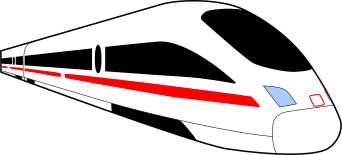
\includegraphics[scale=0.4]{img/analytic_geometry/train}} -- (2,-0.5) node[black, above, midway] {$\vec{v}$} node[sloped, pos=1, anchor=west] {direction};
\draw [decorate, decoration={brace, amplitude=5pt, mirror}, xshift=-2pt, yshift=-2pt] (0,0) -- (2,-0.5) node [midway, below, sloped, xshift=-2pt, yshift=-2pt] {magnitude};
\end{tikzpicture}

\end{center}
\end{frame}


% ---------------------------------------------------------------------slide----
\begin{frame}
\frametitle{Vector representation}
An oriented segment can be located in different places in a Cartesian space.  
However, regardless of where it is located, if the length and the direction of the segment doesn't change, the segment represents always the same vector. 

This allows to represent all vector with the same origin, the origin of the Cartesian coordinate system.
Thus, a vector can be represented by the Cartesian \emph{coordinates} of its final end in any Euclidean space.

\begin{center}
\tikzsetnextfilename{analytic_geometry/vector_coordinates}
\input{img/analytic_geometry/vector_coordinates}
\end{center}
\end{frame}


% ---------------------------------------------------------------------slide----
\begin{frame}
\frametitle{Vector from two points}
Given two points $P$ and $Q$ of a Cartesian space, the vector that starts at $P$ and ends at $Q$ has coordinates 
$\vec{PQ}=Q-P$.

\structure{\bfseries Example} Given the points $P=(2,1)$ and $Q=(3,4)$ in the real plane $\mathbb{R}^2$, the coordinates of the vector that start at $P$ and ends at $Q$ are
\[
\vec{PQ} = Q-P = (3,4)-(2,1) = (3-2,4-1) = (1,3).
\]
\begin{center}
\tikzsetnextfilename{analytic_geometry/vector_from_two_points}
% Author: Alfredo Sánchez Alberca (asalber@ceu.es)
\begin{tikzpicture}[trim axis left, trim axis right]
  \begin{axis}[
    2dfun, 
    xmin=-4, xmax=4,
    ymin=-4, ymax=4,  
    equal axis=true,
    height=4cm,
    ]
    \coordinate (0) at (0,0);
    \coordinate (P) at (2,1);
    \coordinate (Q) at (3,4);
    \draw[->, color1] (O) -- (A) node[midway, below, anchor=west] {$\vec{PQ}=(1,3)$} ;
    \draw[gray, dotted] (P) -- (P|-O);
    \draw[gray, dotted] (P) -- (P-|O);
    \draw[gray, dotted] (Q) -- (Q|-O);
    \draw[gray, dotted] (Q) -- (Q-|O);
  \end{axis}
\end{tikzpicture}

\end{center}
\end{frame}

% 
% % ---------------------------------------------------------------------slide----
% \begin{frame}
% \frametitle{Módulo de un vector}
% \begin{definition}[Módulo de un vector]
% Dado un vector $\mathbf{v}=(v_1,\cdots,v_n)$ de $\mathbb{R}^n$, se define el \emph{módulo} de $\mathbf{v}$ como
% \[
% |\mathbf{v}| = \sqrt{v_1^2+ \cdots + v_n^2}.
% \]
% \end{definition}
% El módulo de un vector coincide con la longitud del segmento que representa al vector.
% 
% \structure{\bfseries Ejemplos} 
% Sea $\mathbf{u}=(3,4)$ un vector en $\mathbb{R}^2$, entonces
% \[
% |\mathbf{u}| = \sqrt{3^2+4^2} = \sqrt{25} = 5
% \]
% Sea $\mathbf{v}=(4,7,4)$ un vector en $\mathbb{R}^3$, entonces
% \[
% |\mathbf{v}| = \sqrt{4^2+7^2+4^2} = \sqrt{81} = 9
% \]
% \end{frame} 
% 
% 
% % ---------------------------------------------------------------------slide----
% \begin{frame}
% \frametitle{Vectores unitarios}
% \begin{definition}[Vector unitario]
% Se dice que un vector $\mathbf{v}$ de $\mathbb{R}^n$ es \emph{unitario} si su módulo es 1, es decir $|\mathbf{v}|=1$.
% \end{definition}
% Especial atención merecen los vectores unitarios que siguen la dirección de los ejes de coordenadas, estos vectores se llaman \emph{vectores coordenados}.
% \begin{columns}
% \begin{column}{.48\textwidth}
% En $\mathbb{R}^2$ los vectores coordenados son 
% \[
% \mathbf{i}=(1,0)\mbox{ y }\mathbf{j}=(0,1)
% \]
% \begin{center}
% \scalebox{1}{\input{img/geometria_analitica/vectores_unitarios_r2}}
% \end{center}
% \end{column}
% \begin{column}{.48\textwidth}
% En $\mathbb{R}^3$ los vectores coordenados son 
% \[
% \mathbf{i}=(1,0,0)\mbox{, }\mathbf{j}=(0,1,0) \mbox{ y } \mathbf{k}=(0,0,1)
% \]
% \begin{center}
% \scalebox{1}{\input{img/geometria_analitica/vectores_unitarios_r3}}
% \end{center}
% \end{column}   
% \end{columns}
% \end{frame} 
% 
% 
% % ---------------------------------------------------------------------slide----
% \begin{frame}
% \frametitle{Suma de vectores}
% \begin{definition}[Suma de vectores]
% Dados dos vectores $\mathbf{u}=(u_1,\cdots,u_n)$ y $\mathbf{v}=(v_1,\cdots,v_n)$ de $\mathbb{R}^n$, se define la
% \emph{suma} de $\mathbf{u}$ y $\mathbf{v}$ como
% \[
% \mathbf{u}+\mathbf{v} = (u_1+v_1,\ldots, u_n+v_n).
% \]
% \end{definition}
% 
% \structure{\bfseries Ejemplo} 
% Sean $\mathbf{u}=(3,1)$ y $\mathbf{v}=(2,3)$ dos vectores en $\mathbb{R}^2$, entonces
% \[
% \mathbf{u}+\mathbf{v} = (3+2,1+3) = (5,4).
% \]
% 
% \begin{center}
% \scalebox{0.8}{\input{img/geometria_analitica/suma_vectores}}
% \end{center}
% \end{frame} 
% 
% 
% %---------------------------------------------------------------------slide----
% \begin{frame}
% \frametitle{Producto de un vector por un escalar}
% \begin{definition}[Producto de un vector por un escalar]
% Dado un vector $\mathbf{v}=(v_1,\cdots,v_n)$ de $\mathbb{R}^n$, y un escalar $a\in \mathbb{R}$, se define el
% \emph{producto} de $a$ por $\mathbf{v}$ como
% \[
% a\mathbf{v} = (av_1,\ldots, av_n).
% \]
% \end{definition}
% \structure{\bfseries Ejemplo}
% Sean el vector $\mathbf{v}=(2,1)$ en $\mathbb{R}^2$ y el escalar $a=2$, entonces
% \[
% a\mathbf{v} = 2(2,1) = (4,2).
% \]
% 
% \begin{center}
% \scalebox{0.8}{\input{img/geometria_analitica/producto_por_escalar}}
% \end{center}
% \end{frame}  
% 
% 
% %---------------------------------------------------------------------slide----
% \begin{frame}
% \frametitle{Expresión de un vector como combinación lineal de los vectores coordenados}
% La suma de vectores y el producto de un vector por un escalar permite expresar cualquier vector como una combinación lineal de los vectores coordenados.
% 
% En el caso del espacio real $\mathbb{R}^3$, cualquier vector $\mathbf{v}=(v_1,v_2,v_3)$ puede expresarse como   
% \[
% \mathbf{v}=(v_1,v_2,v_3) = v_1\mathbf{i}+v_2\mathbf{j}+v_3\mathbf{k}.
% \]
% 
% \begin{center}
% \scalebox{0.8}{\input{img/geometria_analitica/combinacion_lineal_vectores_coordenados}}
% \end{center}
% \end{frame} 
% 
% 
% %---------------------------------------------------------------------slide----
% \begin{frame}
% \frametitle{Producto escalar}
% \begin{definition}[Producto escalar]
% Dados dos vectores $\mathbf{u}=(u_1,\cdots,u_n)$ y $\mathbf{v}=(v_1,\cdots,v_n)$ de $\mathbb{R}^n$, se define el
% \emph{producto escalar} de $\mathbf{u}$ y $\mathbf{v}$ como
% \[
% \mathbf{u}\cdot \mathbf{v} = u_1v_1 + \cdots + u_nv_n.
% \]
% \end{definition}
% \structure{\bfseries Ejemplo} 
% Sean $\mathbf{u}=(3,1)$ y $\mathbf{v}=(2,3)$ dos vectores en $\mathbb{R}^2$, entonces
% \[
% \mathbf{u}\cdot\mathbf{v} = 3\cdot 2 +1\cdot 3 = 9.
% \]
% 
% Se cumple que
% \[
% \mathbf{u}\cdot\mathbf{v} =  |\mathbf{u}||\mathbf{v}|\cos\alpha
% \]
% donde $\alpha$ es el ángulo que forman los vectores.
% \end{frame} 
% 
% 
% %---------------------------------------------------------------------slide----
% \begin{frame}
% \frametitle{Vectores paralelos}
% \begin{definition}[Vectores paralelos]
% Dos vectores $\mathbf{u}$ y $\mathbf{v}$ son \emph{paralelos} si existe un valor $a\in\mathbb{R}$ tal que
% \[
% \mathbf{u} = a\mathbf{v}.
% \]
% \end{definition}
% 
% \structure{\bfseries Ejemplos} 
% Los vectores $\mathbf{u}=(-4,2)$ y $\mathbf{v}=(2,-1)$ en $\mathbb{R}^2$ son paralelos, ya que
% \[
% \mathbf{v}= (-4,2) = -2(2,-1) = -2\mathbf{v}.
% \]
% 
% \end{frame} 
% 
% 
% %---------------------------------------------------------------------slide----
% \begin{frame}
% \frametitle{Vectores ortogonales y ortonormales}
% \begin{definition}[Vectores ortogonales y ortonormales]
% Dos vectores $\mathbf{u}$ y $\mathbf{v}$ son \emph{ortogonales} si su producto escalar es nulo
% \[
% \mathbf{u}\cdot \mathbf{v} = 0.
% \]
% Si además el módulo de ambos vectores es la unidad $|\mathbf{u}|=|\mathbf{v}|=1$, entonces se dice que son \emph{ortonormales}.
% \end{definition}
% 
% Los vectores ortogonales son perpendiculares entre sí, es decir, forman un ángulo de $90^\circ$.
% 
% \structure{\bfseries Ejemplos} 
% Los vectores $\mathbf{u}=(2,1)$ y $\mathbf{v}=(-2,4)$ en $\mathbb{R}^2$ son ortogonales, ya que
% \[
% \mathbf{u}\mathbf{v} = 2\cdot -2 +1\cdot 4 = 0,
% \]
% pero no son ortonormales ya que $|\mathbf{u}| = \sqrt{2^2+1^2} \neq 1$ y  $|\mathbf{v}| = \sqrt{-2^2+4^2} \neq 1$.
% 
% Los vectores $\mathbf{i}=(1,0)$ y $\mathbf{j}=(0,1)$ en $\mathbb{R}^2$ son ortonormales, ya que
% \[
% \mathbf{i}\mathbf{j} = 1\cdot 0 +0\cdot 1 = 0, \quad |\mathbf{i}| = \sqrt{1^2+0^2} = 1,  \quad |\mathbf j| = \sqrt{0^2+1^2} = 1.
% \]
% \end{frame}  
% 
% 
% 
% \subsection{Rectas}
% %---------------------------------------------------------------------slide----
% \begin{frame}
% \frametitle{Ecuación vectorial de la recta}
% \begin{definition}[Ecuación vectorial de la recta]
% Sea $l$ una recta del espacio $\mathbb{R}^n$ y sean $P=(p_1,\ldots,p_n)$ un punto cualquiera de la recta y
% $\mathbf{v}=(v_1,\ldots,v_n)$ un vector cualquiera con la misma dirección que la recta.
% La ecuación
% \[
% l: X= P + t\mathbf{v} = (p_1,\ldots,p_n)+t(v_1,\ldots,v_n) = (p_1+tv_1,\ldots,p_n+tv_n).
% \]
% parametriza a $l$ en función de $t\in \mathbb{R}$, y se conoce como \emph{ecuación vectorial de la recta}.
% \end{definition}
% \begin{columns}
% \begin{column}{.48\textwidth}
% \structure{\bfseries Ejemplo} 
% Considerese la recta del espacio real $\mathbb{R}^3$ que aparece en la gráfica. Un punto de la recta es $P=(1,1,2)$ y un vector director es $\mathbf{v}=(-1,2,2)$, luego su ecuación vectorial es
% \begin{align*}
% l &: X= P + t\mathbf{v} = (1,1,2)+t(-1,2,1) =\\
% &= (1-t,1+2t,2+t)\quad t\in\mathbb{R}.
% \end{align*}
% \end{column}
% \begin{column}{.48\textwidth}
% \begin{center}
% \scalebox{0.8}{\input{img/geometria_analitica/ecuacion_vectorial_recta}}
% \end{center}
% \end{column}
% \end{columns}
% \end{frame} 
% 
% 
% %---------------------------------------------------------------------slide----
% \begin{frame}
% \frametitle{Ecuaciones paramétricas y cartesianas de la recta}
% De la ecuación vectorial de una recta $l: X=P + t\mathbf{v}=(p_1+tv_1,\ldots,p_n+tv_n)$ se obtienen facilmente las coordenadas de los puntos que forman parte de la recta mediante $n$ ecuaciones paramétricas:
% \[
% x_1(t)=p_1+tv_1, \ldots, x_n(t)=p_n+tv_n
% \]
% donde, si $\mathbf{v}$ es un vector cuyas coordenadas son no nulas ($v_i\neq 0$ $\forall i$), se puede despejar el parámetro $t$ en cada una de ellas e igualarlas,
% \[
% \frac{x_1-p_1}{v_1}=\cdots = \frac{x_n-p_n}{v_n}
% \] 
% 
% \structure{\bfseries Ejemplo} 
% Dada la ecuación vectorial de la recta $l: X=(1,1,2)+t(-1,2,1) =(1-t,1+2t,2+t)$ en el espacio real $\mathbb{R^3}$, sus
% ecuaciones paramétricas son
% \[
% x(t) = 1-t, \quad y(t)=1+2t, \quad z(t)=2+t,
% \]
% y sus ecuaciones cartesianas son
% \[
% \frac{x-1}{-1}=\frac{y-1}{2}=\frac{z-2}{1}
% \]
% \end{frame} 
% 
% 
% %---------------------------------------------------------------------slide----
% \begin{frame}
% \frametitle{Ecuación punto-pendiente de una recta en el plano}
% En el caso particular del plano cartesiano $\mathbb{R^2}$, si se tiene una recta con ecuación vectorial $l: X=P+t\mathbf{v}=(x_0,y_0)+t(a,b)
% = (x_0+ta,y_0+tb)$, sus ecuaciones paramétricas son
% \[
% x(t)=x_0+ta,\quad y(t)=y_0+tb
% \]
% y sus ecuación cartesiana es
% \[
% \frac{x-x_0}{a} = \frac{y-y_0}{b}.
% \]  
% A partir de aquí, pasando $b$ multiplicando al otro lado de la ecuación, se obtiene 
% \[
% y-y_0 = \frac{b}{a}(x-x_0) \mbox{ o bien } y-y_0+m(x-x_0),
% \]
% llamando $m=b/a$. Esta ecuación se conoce como ecuación en la forma \emph{punto-pendiente}.
%  
% \end{frame} 
% 
% 
% %---------------------------------------------------------------------slide----
% \begin{frame}
% \frametitle{Pendiente de una recta en el plano}
% \begin{definition}[Pendiente de una recta]
% Dada una recta $l: X=P+t\mathbf{v}$ en el plano real $\mathbb{R}^2$, con vector director $\mathbf{v}=(a,b)$, se define la pendiente de $l$ como $b/a$.
% \end{definition}
% 
% Recordar que dados dos puntos $Q=(x_1,y_1)$ y $Q=(x_2,y_2)$ de la recta $l$, se puede tomar como vector director el vector que los une, que tiene coordenadas $\vec{PQ}=Q-P=(x_2-x_1,y_2-y_1)$, de manera que la pendiente de $l$ será 
% $\dfrac{y_2-y_1}{x_2-x_1}$, es decir, el cociente entre lo que cambia la coordenada $y$ y lo que cambia la coordenada $x$.
% 
% \begin{center}
% \scalebox{0.7}{\input{img/geometria_analitica/pendiente_recta}}
% \end{center}
% \end{frame} 
% 
% 
% 
% \subsection{Planos}
% %---------------------------------------------------------------------slide----
% \begin{frame}
% \frametitle{Ecuación del plano en el espacio real}
% Para llegar a la ecuación de un plano en el espacio real $\mathbb{R}^3$ se puede partir de un punto del plano $P=(x_0,y_0,z_0)$ y de un vector perpendicular al plano $\mathbf{v}=(a,b,c)$. 
% Entonces, para cualquier punto del plano $Q=(x,y,z)$ se cumple que el vector $\vec{PQ} = (x-x_0,y-y_0,z-z_0)$ es ortogonal a $\mathbf{v}$, por lo que su producto escalar se anulará
% \[
% \vec{PQ}\cdot\mathbf{v} = (x-x_0,y-y_0,z-z_0)(a,b,c) = a(x-x_0)+b(y-y_0)+c(z-z_0) = 0.
% \]
% 
% \begin{center}
% \scalebox{0.8}{\input{img/geometria_analitica/ecuacion_plano}}
% \end{center}
% \end{frame} 




% !TEX root = ../calculus_manual.tex
\section{Differential calculus with one variable}
%---------------------------------------------------------------------slide----
\begin{frame}
\frametitle{Differential calculus with one variable}
\tableofcontents[sectionstyle=show/hide,hideothersubsections]
\end{frame}


\subsection{Concept of derivative}
%---------------------------------------------------------------------slide----
\begin{frame}
\frametitle{Increment}
\begin{definition}[Increment of a variable]
An \emph{increment} of a variable $x$ is a change in the value of the variable and is denoted $\Delta x$.
The increment of a variable $x$ along an interval $[a,b]$ is
\[
\Delta x = b-a.
\]
\end{definition}

\begin{definition}[Increment of a function]
The \emph{increment} of a function $y=f(x)$ along an interval $[a,b]\subseteq Dom(f)$ is
\[
\Delta y = f(b)-f(a).
\]
\end{definition}

\textbf{Example} The increment of $x$ along the interval $[2,5]$ is $\Delta x=5-2=3$ and the increment of the function $y=x^2$ along the same interval is $\Delta y=5^2-2^2=21$.
\end{frame}

\begin{frame}
\frametitle{Average rate of change}
The study of a function $y=f(x)$ requires to anderstand how the function changes, that is, how changes the dependent variable $y$ when we change the independent variable $x$.

\begin{definition}[Average rate of change]
The  \emph average rate of change of a function $f$ in an interval $[a,a+\Delta x]\subseteq Dom(f)$, is the quotient between the increment of $y=f(x)$ and the increment of $x$ in that interval, and is denoted
\[
\mbox{ARC}\;f[a,a+\Delta x]=\frac{\Delta y}{\Delta x}=\frac{f(a+\Delta x)-f(a)}{\Delta x}.
\]
\end{definition}
\end{frame}

% %---------------------------------------------------------------------slide----
% \begin{frame}
% \frametitle{Tasa de variación media: Ejemplo}
% Consideremos la función $y=x^2$ que mide el área de un cuadrado de chapa metálica de lado $x$.
%
% Si en un determinado instante el lado del cuadrado es $a$, y sometemos la chapa a un proceso de calentamiento que aumenta el lado del cuadrado una cantidad $\Delta x$, ¿en cuánto se incrementará el área del cuadrado?
% \begin{columns}
% \begin{column}{0.3\textwidth}
% \begin{align*}
% \Delta y &= f(a+\Delta x)-f(a)=(a+\Delta x)^2-a^2=\\
% &= a^2+2a\Delta x+\Delta x^2-a^2=2a\Delta x+\Delta x^2.
% \end{align*}
% \end{column}
% \begin{column}{0.3\textwidth}
% \begin{center}
% \scalebox{1}{\input{img/calculo_diferencial_1_variable/variacion_area_cuadrado}}
% \end{center}
% \end{column}
% \end{columns}
% ¿Cuál será la tasa de variación media del área en el intervalo $[a,a+\Delta x]$?
% \[
% \textrm{TVM}\;f[a,a+\Delta x]=\frac{\Delta y}{\Delta x}=\frac{2a\Delta x+\Delta x^2}{\Delta x}=2a+\Delta x.
% \]
% \end{frame}

%
% %---------------------------------------------------------------------slide----
% \begin{frame}
% \frametitle{Interpretación geométrica de la tasa de variación media}
% La tasa de variación media de $f$ en el intervalo $[a,a+\Delta x]$ es la pendiente de la recta \emph{secante} a $f$ en los puntos $(a,f(a))$ y $(a+\Delta x,f(a+\Delta x))$.
% \begin{center}
% \scalebox{1}{\input{img/calculo_diferencial_1_variable/secante}}
% \end{center}
% \end{frame}
%
%
% %---------------------------------------------------------------------slide----
% \begin{frame}
% \frametitle{Tasa de variación instantánea}
% En muchas ocasiones, es interesante estudiar la tasa de variación que experimenta una función, no en intervalo, sino en
% un punto.
%
% Conocer la tendencia de variación de una función en un instante puede ayudarnos a predecir valores en instantes
% próximos.
%
% \begin{definicion}[Tasa de variación instantánea y derivada]
% Dada una función $y=f(x)$, se llama \emph{tasa de variación instantánea} de $f$ en un punto $a$, al límite de la tasa de
% variación media de $f$ en el intervalo $[a,a+\Delta x]$, cuando $\Delta x$ tiende a 0, y lo notaremos
% \[
% \textrm{TVI}\;f (a)=\lim_{\Delta x\rightarrow 0} \textrm{TVM}\; f[a,a+\Delta x]=\lim_{\Delta x\rightarrow 0}\frac{\Delta y}{\Delta x}=\lim_{\Delta x\rightarrow 0}\frac{f(a+\Delta x)-f(a)}{\Delta x}
% \]
% Cuando este límite existe, se dice que la función $f$ es derivable en el punto $a$, y al valor del mismo se le llama
% derivada de $f$ en $a$, y se nota como
% \[
% f'(a) \mbox{ o bien } \frac{df}{dx}(a)
% \]
% \end{definicion}
% \end{frame}
%
%
% %---------------------------------------------------------------------slide----
% \begin{frame}
% \frametitle{Tasa de variación instantánea: Ejemplo}
% Consideremos de nuevo la función $y=x^2$ que mide el área de un cuadrado de chapa metálica de lado $x$.
%
% Si en un determinado instante el lado del cuadrado es $a$, y sometemos la chapa a un proceso de calentamiento que
% aumenta el lado del cuadrado, ¿cuál es la tasa de variación instantánea del área del cuadrado en dicho instante?
% \begin{align*}
% \textrm{TVI}\;f(a)]&=\lim_{\Delta x\rightarrow 0}\frac{\Delta y}{\Delta x}=\lim_{\Delta x\rightarrow 0}\frac{f(a+\Delta x)-f(a)}{\Delta x} =\\
% &=\lim_{\Delta x\rightarrow 0}\frac{2a\Delta x+\Delta x^2}{\Delta x}=\lim_{\Delta x\rightarrow 0} 2a+\Delta x= 2a.
% \end{align*}
% Así pues,
% \[
% f'(a)=2a,
% \]
% lo que indica que la tendencia de crecimiento el área es del doble del valor del lado.
%
% El signo de $f'(a)$ indica la tendencia de crecimiento de $f$ en el punto $a$:
% \begin{itemize}
% \item[--]  $f'(a)>0$ indica que la tendencia es creciente.
% \item[--]  $f'(a)<0$ indica que la tendencia es decreciente.
% \end{itemize}
% \end{frame}
%
%
% %---------------------------------------------------------------------slide----
% \begin{frame}
% \frametitle{Interpretación geométrica de la tasa de variación instantánea}
% La tasa de variación instantánea de $f$ en el punto $a$ es la pendiente de la recta \emph{tangente} a $f$ en el punto $(a,f(a))$.
% \begin{center}
% \scalebox{1}{\input{img/calculo_diferencial_1_variable/tangente}}
% \end{center}
% \end{frame}
%
%
%
% \subsection{Álgebra de derivadas}
% %---------------------------------------------------------------------slide----
% \begin{frame}
% \frametitle{Propiedades de la derivada}
% Si $y=c$, es una función constante, entonces $y'=0$.
%
% Si $y=x$, es la función identidad, entonces  $y'=1$.
%
% Si $u=f(x)$ y $v=g(x)$ son dos funciones diferenciables, entonces
% \begin{itemize}
% \item $(u+v)'=u'+v'$
% \item $(u-v)'=u'-v'$
% \item $(u\cdot v)'=u'\cdot v+ u\cdot v'$
% \item $\left(\dfrac{u}{v}\right)'=\dfrac{u'\cdot v-u\cdot v'}{v^2}$
% \end{itemize}
% \end{frame}
%
%
% \subsection{Derivada de una función compuesta: La regla de la cadena}
%
% %---------------------------------------------------------------------slide----
% \begin{frame}
% \frametitle{Diferencial de una función compuesta}
% \framesubtitle{La regla de la cadena}
% \begin{teorema}[Regla de la cadena] Si
% $y=f\circ g$ es la composición de dos funciones $y=f(z)$ y $z=g(x)$, entonces
% \[
% (f\circ g)'(x)=f'(g(x))g'(x),
% \]
% \end{teorema}
%
% Resulta sencillo demostrarlo con la notación diferencial
% \[
% \frac{dy}{dx}=\frac{dy}{dz}\frac{dz}{dx}=f'(z)g'(x)=f'(g(x))g'(x).
% \]
%
% \structure{\textbf{Ejemplo}} Si $f(z)=\sen z$ y $g(x)=x^2$, entonces $f\circ g(x)=\sen(x^2)$ y, aplicando la regla de la cadena, su derivada
% vale
% \[
% (f\circ g)'(x)=f'(g(x))g'(x) = \cos g(x) 2x = \cos(x^2)2x.
% \]
% Por otro lado, $g\circ f(z)= (\sin z)^2$ y, de nuevo aplicando la regla de la cadena, su derivada vale
%
% \[
% (g\circ f)'(z)=g'(f(z))f'(z) = 2f(z)\cos z = 2\sen z\cos z.
% \]
% \end{frame}
%
%
%
% \subsection{Derivada de la inversa de una función}
% %---------------------------------------------------------------------slide----
% \begin{frame}
% \frametitle{Derivada de la función inversa}
% \begin{teorema}[Derivada de la inversa]
% Si $y=f(x)$ es una función y $x=f^{-1}(y)$ es su inversa, entonces
% \[
% \left(f^{-1}\right)'(y)=\frac{1}{f'(x)}=\frac{1}{f'(f^{-1}(y))}
% \]
% \end{teorema}
%
% También resulta sencillo de demostrar con la notación diferencial
% \[
% \frac{dx}{dy}=\frac{1}{dy/dx}=\frac{1}{f'(x)}=\frac{1}{f'(f^{-1}(y))}
% \]
%
% \structure{\textbf{Ejemplo}} La inversa de la función exponencial $y=f(x)=e^x$ es el logaritmo neperiano $x=f^{-1}(y)=\ln y$, de modo que
% para calcular la derivada del logaritmo podemos utilizar el teorema de la derivada de la inversa y se tiene
% \[
% \left(f^{-1}\right)'(y)=\frac{1}{f'(x)}=\frac{1}{e^x}=\frac{1}{e^{\ln y}}=\frac{1}{y}.
% \]
% \end{frame}
%
%
% \subsection{Interpretación cinemática de la derivada}
% % ---------------------------------------------------------------------slide----
% \begin{frame}
% \frametitle{Interpretación cinemática de la tasa de variación}
% \framesubtitle{Movimiento rectilineo}
% Supongase que la función $f(t)$ describe la posición de un objeto móvil sobre la recta real en el instante $t$.
% Tomando como referencia el origen de coordenadas $O$ y el vector unitario $\mathbf{i}=(1)$, se puede representar la
% posición $P$ del móvil en cada instante $t$ mediante un vector $\vec{OP}=x\mathbf{i}$ donde $x=f(t)$.
% \begin{center}
% \scalebox{1}{\input{img/calculo_diferencial_1_variable/movimiento_rectilineo}}
% \end{center}
%
% \structure{\textbf{Observación}}
% También tiene sentido pensar en $f$ como una función que mide otras magnitudes como por ejemplo la temperatura de un
% cuerpo, la concentración de un gas o la cantidad de un compuesto en una reacción química en un instante $t$.
% \end{frame}
%
%
% % ---------------------------------------------------------------------slide----
% \begin{frame}
% \frametitle{Interpretación cinemática de la tasa de variación media}
% En este contexto, si se toman los instantes $t=t_0$ y $t=t_0+\Delta t$, ambos del dominio $I$ de $f$, el vector
% \[
% \mathbf{v}_m=\frac{f(t_0+\Delta t)-f(t_0)}{\Delta t}
% \]
% que se conoce como \emph{velocidad media} de la trayectoria $f$ entre los instantes $t_0$ y $t_0+\Delta t$.
%
% \structure{\textbf{Ejemplo}}
% Un vehículo realiza un viaje de Madrid a Barcelona.
% Sea $f$ la función que da la posición el vehículo en cada instante.
% Si el vehículo parte de Madrid (km 0) a las 8 y llega a Barcelona (km 600) a las 14 horas, entonces la velocidad media
% del vehículo en el trayecto es
% \[
% \mathbf{v}_m=\frac{f(14)-f(8)}{14-8}=\frac{600-0}{6} = 100 km/h.
% \]
% \end{frame}
%
%
% % ---------------------------------------------------------------------slide----
% \begin{frame}
% \frametitle{Interpretación cinemática de la derivada}
% Siguiendo en este mismo contexto del movimiento rectilineo, la derivada de $f$ en el instante $t=t_0$ es el vector
% \[
% \mathbf{v}=f'(t_0)=\lim_{\Delta t\rightarrow 0}\frac{f(t_0+\Delta t)-f(t_0)}{\Delta t},
% \]
% que se conoce, siempre que exista el límite, como \emph{velocidad instantánea} o simplemente la \emph{velocidad} de la
% trayectoria $f$ en el instante $t_0$.
%
% Es decir, la derivada de la posición respecto del tiempo, es un campo de vectores que recibe el nombre de
% \emph{velocidad a lo largo de la trayectoria $f$}.
%
% \structure{\textbf{Ejemplo}}
% Siguiendo con el ejemplo anterior, lo que marca el velocímetro en un determinado instante sería el módulo del vector
% velocidad  en ese instante.
% \end{frame}
%
%
% % ---------------------------------------------------------------------slide----
% \begin{frame}
% \frametitle{Generalización al movimiento curvilineo}
% La derivada como velocidad a lo largo de una trayectoria en la recta real puede generalizarse a trayectorias en cualquier
% espacio euclídeo $\mathbb{R}^n$.
%
% Para el caso del plano real $\mathbb{R}^2$, si $f(t)$ describe la posición de un objeto móvil en el plano en el instante
% $t$, tomando como referencia el origen de coordenadas $O$ y los vectores coordenados
% $\{\mathbf{i}=(1,0),\mathbf{j}=(0,1)\}$, se puede representar la posición $P$ del móvil en cada instante $t$ mediante un
% vector $\vec{OP}=x(t)\mathbf{i}+y(t)\mathbf{j}$ cuyas coordenadas
% \[
% \begin{cases}
% x=x(t)\\
% y=y(t)
% \end{cases}
% \quad
% t\in I\subseteq \mathbb{R}
% \]
% se conocen como \emph{funciones coordenadas} de $f$ y se escribe $f(t)=(x(t),y(t))$.
%
% \begin{center}
% \scalebox{0.8}{\input{img/calculo_diferencial_1_variable/movimiento_curvilineo}}
% \end{center}
% \end{frame}
%
%
% % ---------------------------------------------------------------------slide----
% \begin{frame}
% \frametitle{Velocidad en una trayectoria curvilinea en el plano}
% En este contexto de una trayectoria $f(t)=(x(t),y(t))$ en el plano real $\mathbb{R}^2$, para un instante $t=t_0$, si existe el vector
% \[
% \mathbf{v} = \lim_{\Delta t\rightarrow 0} \frac{f(t_0+\Delta t)-f(t_0)}{\Delta t},
% \]
% entonces $f$ es derivable en el instante $t=t_0$ y el vector $\mathbf{v}=f'(t_0)$ se conoce como \emph{velocidad} de $f$ en ese instante.
%
% Como $f(t_0)=(x(t),y(t))$,
% \begin{align*}
% f'(t)&=\lim_{\Delta t\rightarrow 0} \frac{f(t_0+\Delta t)-f(t_0)}{\Delta t} = \lim_{\Delta t\rightarrow 0} \frac{(x(t_0+\Delta t),y(t_0+\Delta t))-(x(t_0),y(t_0))}{\Delta t} =\\
% &=  \lim_{\Delta t\rightarrow 0} \left(\frac{x(t_0+\Delta t)-x(t_0)}{\Delta t},\frac{y(t_0+\Delta t)-y(t_0)}{\Delta t}\right) =\\
% &= \left(\lim_{\Delta t\rightarrow 0}\frac{x(t_0+\Delta t)-x(t_0)}{\Delta t},\lim_{\Delta t\rightarrow 0}\frac{y(t_0+\Delta t)-y(t_0)}{\Delta t}\right) =
% (x'(t_0),y'(t_0)).
% \end{align*}
% luego
% \[
% \mathbf{v} = x'(t_0)\mathbf{i}+y'(t_0)\mathbf{j}.
% \]
% \end{frame}
%
%
% % ---------------------------------------------------------------------slide----
% \begin{frame}
% \frametitle{Velocidad en una trayectoria curvilinea en el plano}
% \framesubtitle{Ejemplo}
% Dada la trayectoria $f(t) = (\cos t,\sen t)$, $t\in \mathbb{R}$, cuya imagen es la circunferencia de centro el origen
% de coordenas y radio 1, sus funciones coordenadas son $x(t) = \cos t$, $y(t) = \sen t$, $t\in \mathbb{R}$, y su velocidad es
% \[
% \mathbf{v}=f'(t)=(x'(t),y'(t))=(-\sen t, \cos t).
% \]
% En el instante $t=\pi/4$, el móvil estará en la posición $f(\pi/4) = (\cos(\pi/4),\sen(\pi/4)) =(\sqrt{2}/2,\sqrt{2}/2)$
% y se moverá con una velocidad $\mathbf{v}=f'(\pi/4)=(-\sen(\pi/4),\cos(\pi/4))=(-\sqrt{2}/2,\sqrt{2}/2)$.
% \begin{center}
% \scalebox{0.8}{\input{img/calculo_diferencial_1_variable/circunferencia}}
% \end{center}
% Obsérvese que el módulo del vector velocidad siempre será 1 ya que
% $|\mathbf{v}|=\sqrt{(-\sen t)^2+(\cos t)^2}=1$.
% \end{frame}
%
%
%
% \subsection{Recta tangente a una trayectoria}
% % ---------------------------------------------------------------------slide----
% \begin{frame}
% \frametitle{Recta tangente a una trayectoria en el plano}
% Los vectores paralelos a la velocidad $\mathbf{v}$ se denominan \emph{vectores tangentes} a la trayectoria
% $f$ en el instante $t=t_0$, y la recta que pasa por $P=f(t_0)$ dirigida por $\mathbf{v}$ es la recta tangente a $f$ cuando
% $t=t_0$.
% \begin{definicion}[Recta tangente a una trayectoria]
% Dada una trayectoria $f$ sobre el plano real $\mathbb{R}^2$, se llama \emph{recta tangente} a $f$ para $t=t_0$ a la
% recta de ecuación
% \[
% l: (x,y)= f(t_0)+tf'(t_0) = (x(t_0),y(t_0))+t(x'(t_0),y'(t_0)) = (x(t_0)+tx'(t_0),y(t_0)+ty'(t_0)).
% \]
% \end{definicion}
% \structure{\texbf{Ejemplo}}
% Se ha visto que para la trayectoria $f(t) = (\cos t,\sen t)$, $t\in \mathbb{R}$, cuya imagen es la circunferencia de
% centro el origen de coordenas y radio 1, en el instante $t=\pi/4$ la posición del móvil era
% $f(\pi/4)=(\sqrt{2}/2,\sqrt{2}/2)$ y su velocidad $\mathbf{v}=(-\sqrt{2}/2,\sqrt{2}/2)$, de modo que la recta tangente a
% $f$ en ese instante es
% \[
% l: X=f(\pi/4)+t\mathbf{v} =
% \left(\frac{\sqrt{2}}{2},\frac{\sqrt{2}}{2}\right)+t\left(\frac{-\sqrt{2}}{2},\frac{\sqrt{2}}{2}\right) =
% \left(\frac{\sqrt{2}}{2}-t\frac{\sqrt{2}}{2},\frac{\sqrt{2}}{2}+t\frac{\sqrt{2}}{2}\right).
% \]
% \end{frame}
%
%
% % ---------------------------------------------------------------------slide----
% \begin{frame}
% \frametitle{Recta tangente a una trayectoria en el plano}
% De la ecuación vectorial de la recta tangente a $f$ para $t=t_0$, se obtiene que sus funciones cartesianas son
% \[
% \begin{cases}
% x=x(t_0)+tx'(t_0)\\
% y=y(t_0)+ty'(t_0)
% \end{cases}
% \quad t\in \mathbb{R},
% \]
% y despejando $t$ en ambas ecuaciones e igualando se llega a la ecuación cartesiana de la recta tangente
% \[
% \frac{x-x(t_0)}{x'(t_0)}=\frac{y-y(t_0)}{y'(t_0)},
% \]
% si $x'(t_0)\neq 0$ e $y'(t_0)\neq 0$, y de ahí a la ecuación en la forma punto-pendiente
% \[
% y-y(t_0)=\frac{y'(t_0)}{x'(t_0)}(x-x(t_0)).
% \]
% \structure{\texbf{Ejemplo}}
% Partiendo de la ecuación vectorial de la tangente del ejemplo anterior
% $l=\left(\frac{\sqrt{2}}{2}-t\frac{\sqrt{2}}{2},\frac{\sqrt{2}}{2}+t\frac{\sqrt{2}}{2}\right)$, su ecuación cartesiana
% es
% \[
% \frac{x-\sqrt{2}/2}{-\sqrt{2}/2} = \frac{y-\sqrt{2}/2}{\sqrt{2}/2}\Rightarrow y-\sqrt{2}/2 =
% \frac{-\sqrt{2}/2}{\sqrt{2}/2}(x-\sqrt{2}/2) \Rightarrow y=-x+\sqrt{2}.
% \]
% \end{frame}
%
%
% % ---------------------------------------------------------------------slide----
% \begin{frame}
% \frametitle{Recta normal a una trayectoria en el plano}
% Se ha visto que la recta tangente a una trayectoria $f$ cuando $t=t_0$ es la recta que pasa por el punto el punto
% $P=f(t_0)$ dirigida por el vector velocidad $\mathbf{v}=f'(t_0)=(x'(t_0),y'(t_0))$. Si en lugar de tomar ese vector se
% toma como vector director el vector $\mathbf{w}=(y'(t_0),-x'(t_0))$, que es ortogonal a $\mathbf{v}$, se obtiene otra
% recta que se conoce como \emph{recta normal} a la trayectoria $f$ cuanto $t=t_0$.
% \begin{definicion}[Recta normal a una trayectoria]
% Dada una trayectoria $f$ sobre el plano real $\mathbb{R}^2$, se llama \emph{recta normal} a $f$ para $t=t_0$ a la recta de ecuación
% \[
% l: (x,y)=(x(t_0),y(t_0))+t(y'(t_0),-x'(t_0)) = (x(t_0)+ty'(t_0),y(t_0)-tx'(t_0)).
% \]
% \end{definicion}
% Su ecuación cartesiana es
% \[
% \frac{x-x(t_0)}{y'(t_0)} = \frac{y-y(t_0)}{-x'(t_0)},
% \]
% y su ecuación en la forma punto pendiente
% \[
% y-y(t_0) = \frac{-x'(t_0)}{y'(t_0)}(x-x(t_0)).
% \]
% La recta normal es perpendicular a la recta tangente ya que sus vectores directores son ortogonales.
% \end{frame}
%
%
% % ---------------------------------------------------------------------slide----
% \begin{frame}
% \frametitle{Recta normal a una trayectoria en el plano}
% \framesubtitle{Ejemplo}
% Siguiendo con el ejemplo de la trayectoria $f(t) = (\cos t,\sen t)$, $t\in \mathbb{R}$, la recta normal en el instante $t=\pi/4$ es
% \begin{align*}
% l&: (x,y)=(\cos(\pi/2),\sen(\pi/2))+t(\cos(\pi/2),\sen(\pi/2)) =\\
% & \left(\frac{\sqrt{2}}{2},\frac{\sqrt{2}}{2}\right)+t\left(\frac{\sqrt{2}}{2},\frac{\sqrt{2}}{2}\right)
% =\left(\frac{\sqrt{2}}{2}+t\frac{\sqrt{2}}{2},\frac{\sqrt{2}}{2}+t\frac{\sqrt{2}}{2}\right),
% \end{align*}
% y su ecuación cartesiana es
% \[
% \frac{x-\sqrt{2}/2}{\sqrt{2}/2} = \frac{y-\sqrt{2}/2}{\sqrt{2}/2}\Rightarrow y-\sqrt{2}/2 = \frac{\sqrt{2}/2}{\sqrt{2}/2}(x-\sqrt{2}/2) \Rightarrow y=x.
% \]
% \begin{center}
% \scalebox{0.8}{\input{img/calculo_diferencial_1_variable/circunferencia_tangente_normal}}
% \end{center}
% \end{frame}
%
%
% % ---------------------------------------------------------------------slide----
% \begin{frame}
% \frametitle{Rectas tangente y normal a una función}
% Un caso particular de las recta tangente y normal a una trayectoria es son la recta tangente y normal a una función de una variable real.
% Si se tiene la función $y=f(x)$, $x\in I\subseteq \mathbb{R}$, una trayectoria que traza la gráfica de $f$ es
% \[
% g(t) = (t,f(t))  \quad t\in I,
% \]
% y su velocidad es
% \[
% g'(t) = (1,f'(t)),
% \]
% de modo que la recta tangente para $t=x_0$ es
% \[
% \frac{x-x_0}{1} = \frac{y-f(x_0)}{f'(x_0)} \Rightarrow y-f(x_0) = f'(x_0)(x-x_0),
% \]
% y la recta normal es
% \[
% \frac{x-x_0}{f'(x_0)} = \frac{y-f(x_0)}{-1} \Rightarrow y-f(x_0) = \frac{-1}{f'(x_0)}(x-x_0),
% \]
% % \begin{center}
% % \scalebox{1}{\input{img/calculo_diferencial_1_variable/tangente_normal}}
% % \end{center}
% \end{frame}
%
%
% % ---------------------------------------------------------------------slide----
% \begin{frame}
% \frametitle{Rectas tangente y normal a una función}
% \framesubtitle{Ejemplo}
% Dada la función $y=f(x)=x^2$, la trayectoria que dibuja la gráfica de esta función es $g(t)=(t,t^2)$ y su velocidad es
% $g'(t)=(1,2t)$, de modo que en el punto $(1,1)$, que se alcanza en el instante $t=1$, la recta tangente es
% \[
% \frac{x-1}{1} = \frac{y-1}{2} \Rightarrow y-1 = 2(x-1) \Rightarrow y = 2x-1,
% \]
% y la recta normal es
% \[
% \frac{x-1}{2} = \frac{y-1}{-1} \Rightarrow y-1 = \frac{-1}{2}(x-1) \Rightarrow y = \frac{-x}{2}+\frac{3}{2}.
% \]
% \begin{center}
% \scalebox{0.8}{\input{img/calculo_diferencial_1_variable/parabola_tangente_normal}}
% \end{center}
% \end{frame}
%
%
% % ---------------------------------------------------------------------slide----
% \begin{frame}
% \frametitle{Recta tangente a una trayectoria en el espacio}
% El concepto de recta tangente a una trayectoria en el plano real puede extenderse fácilmente a trayectorias en el espacio real $\mathbb{R}^3$.
%
% Si $f(t)=(x(t),y(t),z(t))$, $t\in I\subseteq \mathbb{R}$, es una trayectoria en el espacio real $\mathbb{R}^3$, entonces
% el móvil que recorre esta trayectoria en el instante $t=t_0$, ocupará la posición $P=(x(t_0),y(t_0),z(t_0))$ y tendrá una velocidad $\mathbf{v}=f'(t)=(x'(t),y'(t),z'(t))$, de manera que la recta tangente a $f$ en ese instante será
% \begin{align*}
% l&: (x,y,z)=(x(t_0),y(t_0),z(t_0))+t(x'(t_0),y'(t_0),z'(t_0)) =\\
% &= (x(t_0)+tx'(t_0),y(t_0)+ty'(t_0),z(t_0)+tz'(t_0)),
% \end{align*}
% cuyas ecuaciones cartesianas son
% \[
% \frac{x-x(t_0)}{x'(t_0)}=\frac{y-y(t_0)}{y'(t_0)}=\frac{z-z(t_0)}{z'(t_0)},
% \]
% siempre que $x'(t_0)\neq 0$, $y'(t_0)\neq 0$ y $z'(t_0)\neq 0$.
% \end{frame}
%
%
% % ---------------------------------------------------------------------slide----
% \begin{frame}
% \frametitle{Recta tangente a una trayectoria en el espacio}
% \framesubtitle{Ejemplo}
% Dada la trayectoria del espacio $f(t)=(\cos t, \sen t, t)$, $t\in \mathbb{R}$, en el instante $t=\pi/2$, la trayectoria
% pasará por el punto
% \[
% f(\pi/2)=(\cos(\pi/2),\sen(\pi/2),\pi/2)=(0,1,\pi/2),
% \] con una velocidad
% \[
% \mathbf{v}=f'(\pi/2)=(-\sen(\pi/2),\cos(\pi/2), 1)=(-1,0,1),
% \] y la
% tangente en ese punto es
% \[
% l:(x,y,z)=(0,1,\pi/2)+t(-1,0,1) = (-t,1,t+\pi/2).
% \]
% \begin{center}
% \scalebox{0.8}{\input{img/calculo_diferencial_1_variable/tangente_trayectoria_espacio}}
% \end{center}
% \end{frame}
%
%
% \subsection{Estudio del crecimiento de una función}
% %---------------------------------------------------------------------slide----
% \begin{frame}
% \frametitle{Estudio del crecimiento de una función}
% La principal aplicación de la derivada es el estudio del crecimiento de una función mediante el signo de la derivada.
% \begin{teorema}
% Si $f$ es una función cuya derivada existe en un intervalo $I$, entonces:
% \begin{itemize}
% \item Si $\forall x\in I\ f'(x)\geq 0$ entonces $f$ es creciente en el intervalo $I$.
% \item Si $\forall x\in I\ f'(x)\leq 0$ entonces $f$ es decreciente en el intervalo $I$.
% \end{itemize}
% \end{teorema}
% \structure{\textbf{Ejemplo}}
% La función $f(x)=x^3$ es creciente en todo $\mathbb{R}$ ya que $\forall x\in \mathbb{R}\
% f'(x)\geq 0$. \vskip .5cm
% \textbf{Observación}. \emph{Una función puede ser creciente o decreciente en un intervalo y no tener derivada.}
% \end{frame}
%
%
% %---------------------------------------------------------------------slide----
% \begin{frame}
% \frametitle{Estudio del crecimiento de una función}
% \framesubtitle{Ejemplo}
% Consideremos la función $f(x)=x^4-2x^2+1$. Su derivada $f'(x)=4x^3-4x$ está definida en todo $\mathbb{R}$ y es continua.
% \begin{center}
% \scalebox{1}{\input{img/calculo_diferencial_1_variable/estudio_crecimiento}}
% \end{center}
% \end{frame}
%
%
% \subsection{Determinación de los extremos relativos de una función}
% %---------------------------------------------------------------------slide----
% \begin{frame}
% \frametitle{Determinación de extremos relativos de una función}
% Como consecuencia del resultado anterior, la derivada también sirve para determinar los extremos relativos de una función.
% \begin{teorema}[Criterio de la primera derivada]
% Sea $f$ es una función cuya derivada existe en un intervalo $I$, y sea $x_0\in I$ tal que $f'(x_0)=0$, entonces:
% \begin{itemize}
% \item Si existe un $\delta>0$ tal que $\forall x\in(x_0-\delta,x_0)\ f'(x)>0$ y $\forall x\in(x_0,x_0+\delta)\ f'(x)<0$ entonces $f$ tiene un \emph{máximo relativo} en $x_0$.
% \item Si existe un $\delta>0$ tal que $\forall x\in(x_0-\delta,x_0)\ f'(x)<0$ y $\forall x\in(x_0,x_0+\delta)\ f'(x)>0$ entonces $f$ tiene un \emph{mínimo relativo} en $x_0$.
% \item Si existe un $\delta>0$ tal que $\forall x\in(x_0-\delta,x_0)\ f'(x)>0$ y $\forall x\in(x_0,x_0+\delta)\ f'(x)>0$ entonces $f$ tiene un \emph{punto de inflexión creciente} en $x_0$.
% \item Si existe un $\delta>0$ tal que $\forall x\in(x_0-\delta,x_0)\ f'(x)<0$ y $\forall x\in(x_0,x_0+\delta)\ f'(x)<0$ entonces $f$ tiene un \emph{punto de inflexión decreciente} en $x_0$.
% \end{itemize}
% \end{teorema}
% Los puntos donde se anula la derivada de una función se denominan \emph{puntos críticos}.
%
% %\textbf{Observación}. \emph{La anulación de la derivada es una condición necesaria pero no suficiente para la existencia de un extremo relativo en un punto.}
%
% %\structure{\textbf{Ejemplo}} La función $f(x)=x^3$ tiene derivada $f'(x)=3x^2$ y por tanto tiene un punto crítico en $x=0$, pero no tiene un extremo relativo en el 0, sino un punto de inflexión.
% \end{frame}
%
%
% %---------------------------------------------------------------------slide----
% \begin{frame}
% \frametitle{Determinación de extremos relativos de una función}
% \framesubtitle{Ejemplo}
% Consideremos de nuevo la función $f(x)=x^4-2x^2+1$.
% Su derivada $f'(x)=4x^3-4x$ está definida en todo $\mathbb{R}$ y es continua.
% \begin{center}
% \scalebox{1}{\input{img/calculo_diferencial_1_variable/estudio_extremos}}
% \end{center}
% \end{frame}
%
%
% \subsection{Estudio de la concavidad de una función}
% %---------------------------------------------------------------------slide---
% \begin{frame}
% \frametitle{Estudio de la concavidad de una función}
% La concavidad de una función puede estudiarse mediante el signo de la segunda derivada.
% \begin{teorema}[Criterio de la segunda derivada]
% Si $f$ es una función cuya segunda derivada existe en un intervalo $I$, entonces:
% \begin{itemize}
% \item Si $\forall x\in I\ f''(x)\geq 0$ entonces $f$ es cóncava en el intervalo $I$.
% \item Si $\forall x\in I\ f''(x)\leq 0$ entonces $f$ es convexa en el intervalo $I$.
% \end{itemize}
% \end{teorema}
%
% \structure{\textbf{Ejemplo}} La función $f(x)=x^2$ tiene segunda derivada $f''(x)=2>0$ y por tanto es cóncava en todo $\mathbb{R}$.
% \vskip .5cm
% \textbf{Observación}. \emph{Una función puede ser cóncava o convexa en un intervalo y no tener derivada.}
% \end{frame}
%
%
% %---------------------------------------------------------------------slide----
% \begin{frame}
% \frametitle{Estudio de la concavidad de una función}
% \framesubtitle{Ejemplo}
% Consideremos de nuevo la función $f(x)=x^4-2x^2+1$. Su segunda derivada $f''(x)=12x^2-4$ está definida en todo $\mathbb{R}$ y es continua.
% \begin{center}
% \scalebox{1}{\input{img/calculo_diferencial_1_variable/estudio_concavidad}}
% \end{center}
% \end{frame}
%
%
%
% \subsection{Polinomios de Taylor}
% %---------------------------------------------------------------------slide----
% \begin{frame}
% \frametitle{Aproximación de una función mediante un polinomio}
% Una apliación muy útil de la derivada es la aproximación de funciones mediante polinomios.
%
% Los polinomios son funciones sencillas de calcular (mediante sumas y productos), que tienen muy buenas propiedades:
% \begin{itemize}
% \item Están definidos en todos los números reales.
% \item Son funciones continuas.
% \item Son derivables hasta cualquier orden y sus derivadas son continuas.
% \end{itemize}
%
% \begin{block}{Objetivo}
% Aproximar una función $f(x)$ mediante un polinomio $p(x)$ cerca de un valor $x=x_0$.
% \end{block}
%
% \end{frame}
%
%
% %---------------------------------------------------------------------slide----
% \begin{frame}
% \frametitle{Aproximación mediante un polinomio de grado 0}
% Un polinomio de grado 0 tiene ecuación
% \[
% p(x) = c_0,
% \]
% donde $c_0$ es una constante.
%
% Como el polinomio debe valer lo que la función en el punto $x_0$, debe cumplir
% \[p(x_0) = c_0 = f(x_0).\]
%
% En consecuencia, el polinomio de grado 0 que mejor aproxima a $f$ en un entorno de $x_0$ es
% \[p(x) = f(x_0).\]
% \end{frame}
%
%
% %---------------------------------------------------------------------slide----
% \begin{frame}
% \frametitle{Aproximación mediante un polinomio de grado 0}
% \begin{center}
% \scalebox{1}{\input{img/aplicaciones_derivada/polinomio_grado_0}}
% \end{center}
% \end{frame}
%
%
% %---------------------------------------------------------------------slide----
% \begin{frame}
% \frametitle{Aproximación mediante un polinomio de grado 1}
% Un polinomio de grado 1 es una recta y tiene ecuación
% \[
% p(x) = c_0+c_1x,
% \]
% aunque también puede escribirse
% \[
% p(x) = c_0+c_1(x-x_0).
% \]
%
% De entre todos los polinomios de grado 1, el que mejor aproxima a $f$ en entorno de $x_0$ será el que cumpla las dos condiciones siguientes:
% \begin{itemize}
% \item[\structure{1-}] $p$ y $f$ valen lo mismo en $x_0$: $p(x_0) = f(x_0)$,
% \item[\structure{2-}] $p$ y $f$ tienen la misma tasa de crecimiento en $a$: $p'(x_0) = f'(x_0)$.
% \end{itemize}
% Esta última condición nos asegura que en un entorno de $x_0$, $p$ y $f$ tienen aproximadamente la misma tendencia de crecimiento, pero requiere que la función $f$ sea derivable en $x_0$.
% \end{frame}
%
%
% %---------------------------------------------------------------------slide----
% \begin{frame}
% \frametitle{La recta tangente: Mejor aproximación de grado 1}
% Imponiendo las condiciones anteriores tenemos
% \begin{itemize}
% \item[\structure{1-}] $p(x)=c_0+c_1(x-x_0) \Rightarrow p(x_0)=c_0+c_1(x_0-x_0)=c_0=f(x_0)$,
% \item[\structure{2-}] $p'(x)=c_1 \Rightarrow p'(x_0)=c_1=f'(x_0)$.
% \end{itemize}
%
% Así pues, el polinomio de grado 1 que mejor aproxima a $f$ en un entorno de $x_0$ es
% \[
% p(x) = f(x_0)+f '(x_0)(x-x_0),
% \]
% que resulta ser la recta tangente a $f$ en el punto $(x_0,f(x_0))$.
% \end{frame}
%
%
% %---------------------------------------------------------------------slide----
% \begin{frame}
% \frametitle{Aproximación mediante un polinomio de grado 1}
% \begin{center}
% \scalebox{1}{\input{img/aplicaciones_derivada/polinomio_grado_1}}
% \end{center}
% \end{frame}
%
%
% %---------------------------------------------------------------------slide----
% \begin{frame}
% \frametitle{Aproximación mediante un polinomio de grado 2}
% Un polinomio de grado 2 es una parábola y tiene ecuación
% \[
% p(x) = c_0+c_1x+c_2x^2,
% \]
% aunque también puede escribirse
% \[
% p(x) = c_0+c_1(x-x_0)+c_2(x-x_0)^2.
% \]
%
% De entre todos los polinomio de grado 2, el que mejor aproxima a $f$ en entorno de $x_0$ será el que cumpla las tres condiciones siguientes:
% \begin{itemize}
% \item[\structure{1-}] $p$ y $f$ valen lo mismo en $x_0$: $p(x_0) = f(x_0)$,
% \item[\structure{2-}] $p$ y $f$ tienen la misma tasa de crecimiento en $x_0$: $p'(x_0) = f'(x_0)$.
% \item[\structure{3-}] $p$ y $f$ tienen la misma curvatura en $x_0$: $p''(x_0)=f''(x_0)$.
% \end{itemize}
% Esta última condición requiere que la función $f$ sea dos veces derivable en $x_0$.
% \end{frame}
%
%
% %---------------------------------------------------------------------slide----
% \begin{frame}
% \frametitle{Mejor polinomio de grado 2}
% Imponiendo las condiciones anteriores tenemos
% \begin{itemize}
% \item[\structure{1-}] $p(x)=c_0+c_1(x-x_0)+c_2(x-x_0)^2 \Rightarrow p(x_0)=c_0=f(x_0)$,
% \item[\structure{2-}] $p'(x)=c_1+2c_2(x-x_0) \Rightarrow p'(x_0)=c_1+2c_2(x_0-x_0)=c_1=f'(x_0)$,
% \item[\structure{3-}] $p''(x)=2c_2 \Rightarrow p''(x_0)=2c_2=f''(x_0) \Rightarrow c_2=\frac{f''(x_0)}{2}$.
% \end{itemize}
%
% Así pues, el polinomio de grado 2 que mejor aproxima a $f$ en un entorno de $x_0$ es
% \[
% p(x) = f(x_0)+f'(x_0)(x-x_0)+\frac{f''(x_0)}{2}(x-x_0)^2.
% \]
% \end{frame}
%
%
% %---------------------------------------------------------------------slide----
% \begin{frame}
% \frametitle{Aproximación mediante un polinomio de grado 2}
% \begin{center}
% \scalebox{1}{\input{img/aplicaciones_derivada/polinomio_grado_2}}
% \end{center}
% \end{frame}
%
%
% %---------------------------------------------------------------------slide----
% \begin{frame}
% \frametitle{Aproximación mediante un polinomio de grado $n$}
% Un polinomio de grado $n$ tiene ecuación
% \[p(x) = c_0+c_1x+c_2x^2+\cdots +c_nx^n,\]
% aunque también puede escribirse
% \[p(x) = c_0+c_1(x-x_0)+c_2(x-x_0)^2+\cdots +c_n(x-x_0)^n.\]
%
% De entre todos los polinomio de grado $n$, el que mejor aproxima a $f$ en entorno de $x_0$ será el que cumpla las $n+1$ condiciones siguientes:
% \begin{itemize}
% \item[\structure{1-}] $p(x_0) = f(x_0)$,
% \item[\structure{2-}] $p'(x_0) = f'(x_0)$,
% \item[\structure{3-}] $p''(x_0)=f''(x_0)$,
% \item[] $\cdots$
% \item[\structure{n+1-}] $p^{(n}(x_0)=f^{(n}(x_0)$.
% \end{itemize}
% \alert{Obsérvese que para que se cumplan estas condiciones es necesario que $f$ sea $n$ veces derivable en $x_0$.}
% \end{frame}
%
%
% %---------------------------------------------------------------------slide----
% \begin{frame}
% \frametitle{Cálculo de los coeficientes del polinomio de grado $n$}
% Las sucesivas derivadas de $p$ valen
% \begin{align*}
% p(x) &= c_0+c_1(x-x_0)+c_2(x-x_0)^2+\cdots +c_n(x-x_0)^n,\\
% p'(x)& = c_1+2c_2(x-x_0)+\cdots +nc_n(x-x_0)^{n-1},\\
% p''(x)& = 2c_2+\cdots +n(n-1)c_n(x-x_0)^{n-2},\\
% \vdots\ \
% \\
% p^{(n}(x)&= n(n-1)(n-2)\cdots 1 c_n=n!c_n.
% \end{align*}
%
% Imponiendo las condiciones anteriores se tiene
% \begin{itemize}
% \item[\structure{1-}] $p(x_0) = c_0+c_1(x_0-x_0)+c_2(x_0-x_0)^2+\cdots +c_n(x_0-x_0)^n=c_0=f(x_0)$,
% \item[\structure{2-}] $p'(x_0) = c_1+2c_2(x_0-x_0)+\cdots +nc_n(x_0-x_0)^{n-1}=c_1=f'(x_0)$,
% \item[\structure{3-}] $p''(x_0) = 2c_2+\cdots +n(n-1)c_n(x_0-x_0)^{n-2}=2c_2=f''(x_0)\Rightarrow c_2=f''(x_0)/2$,
% \item[] $\cdots$
% \item[\structure{n+1-}] $p^{(n}(x_0)=n!c_n=f^{(n}(x_0)=c_n=\frac{f^{(n}(x_0)}{n!}$.
% \end{itemize}
% \end{frame}
%
%
% %---------------------------------------------------------------------slide----
% \begin{frame}
% \frametitle{Polinomio de Taylor de orden $n$}
% \begin{definicion}[Polinomio de Taylor de orden $n$ para $f$ en el punto $a$]
% Dada una función $f$, $n$ veces derivable en $x=x_0$, se define el \emph{polinomio de Taylor} de orden $n$ para $f$ en $x_0$ como
% \begin{align*}
% p_{f,x_0}^n(x)&=f(x_0)+f'(x_0)(x-x_0)+\frac{f''(x_0)}{2}(x-x_0)^2+\cdots +\frac{f^{(n}(x_0)}{n!}(x-x_0)^n = \\ &=\sum_{i=0}^{n}\frac{f^{(i}(x_0)}{i!}(x-x_0)^i,
% \end{align*}
% o bien, escribiendo $x=x_0+h$
% \[
% p_f^n(x_0+h)&=f(x_0)+f'(x_0)h+\frac{f''(x_0)}{2}h^2+\cdots +\frac{f^{(n}(x_0)}{n!}h^n =\sum_{i=0}^{n}\frac{f^{(i}(x_0)}{i!}h^i,
% \]
% \end{definicion}
%
% El polinomio de Taylor de orden $n$ para $f$ en $x_0$ es el polinomio de orden $n$ que mejor aproxima a $f$ alrededor de $x_0$, ya que es el único que cumple las $n+1$ condiciones anteriores.
% \end{frame}
%
%
% %---------------------------------------------------------------------slide----
% \begin{frame}
% \frametitle{Cálculo del polinomio de Taylor}
% \framesubtitle{Ejemplo}
% Vamos a aproximar la función $f(x)=\log x$ en un entorno del punto $1$ mediante un polinomio de grado $3$.
%
% La ecuación del polinomio de Taylor de orden $3$ para $f$ en el punto $1$ es
% \[
% p_{f,1}^3(x)=f(1)+f'(1)(x-1)+\frac{f''(1)}{2}(x-1)^2+\frac{f'''(1)}{3!}(x-1)^3.
% \]
% Calculamos las tres primeras derivadas de $f$ en $1$:
% \[
% \begin{array}{lll}
% f(x)=\log x & \quad & f(1)=\log 1 =0,\\
% f'(x)=1/x & & f'(1)=1/1=1,\\
% f''(x)=-1/x^2 & & f''(1)=-1/1^2=-1,\\
% f'''(x)=2/x^3 & & f'''(1)=2/1^3=2.
% \end{array}
% \]
% Sustituyendo en la ecuación del polinomio se tiene
% \[
% p_{f,1}^3(x)=0+1(x-1)+\frac{-1}{2}(x-1)^2+\frac{2}{3!}(x-1)^3= \frac{2}{3}x^3-\frac{3}{2}x^2+3x-\frac{11}{6}.
% \]
% \end{frame}
%
%
% %---------------------------------------------------------------------slide----
% \begin{frame}
% \frametitle{Polinomios de Taylor para la función logaritmo}
% \begin{center}
% \scalebox{1}{\input{img/aplicaciones_derivada/polinomio_taylor_logaritmo}}
% \end{center}
% \end{frame}
%
%
% %---------------------------------------------------------------------slide----
% \begin{frame}
% \frametitle{Polinomio de Mc Laurin de orden $n$}
% La ecuación del polinomio de Taylor se simplifica cuando el punto en torno al cual queremos aproximar es el $0$.
% \begin{definicion}[Polinomio de Mc Laurin de orden $n$ para $f$]
% Dada una función $f$, $n$ veces derivable en $0$, se define el \emph{polinomio de Mc Laurin} de orden $n$ para $f$ como
% \begin{align*}
% p_{f,0}^n(x)&=f(0)+f'(0)x+\frac{f''(0)}{2}x^2+\cdots +\frac{f^{(n}(0)}{n!}x^n = \\ &=\sum_{i=0}^{n}\frac{f^{(i}(0)}{i!}x^i.
% \end{align*}
% \end{definicion}
% \end{frame}
%
%
% %---------------------------------------------------------------------slide----
% \begin{frame}
% \frametitle{Cálculo del polinomio de Mc Laurin}
% \framesubtitle{Ejemplo}
% Vamos a aproximar la función $f(x)=\sen x$ en un entorno del punto $0$ mediante un polinomio de grado $3$.
%
% La ecuación del polinomio de Mc Laurin de orden $3$ para $f$ es
% \[
% p_{f,0}^3(x)=f(0)+f'(0)x+\frac{f''(0)}{2}x^2+\frac{f'''(0)}{3!}x^3.
% \]
% Calculamos las tres primeras derivadas de $f$ en $0$:
% \[
% \begin{array}{lll}
% f(x)=\sen x & \quad & f(0)=\sen 0 =0,\\
% f'(x)=\cos x & & f'(0)=\cos 0=1,\\
% f''(x)=-\sen x & & f''(0)=-\sen 0=0,\\
% f'''(x)=-\cos x & & f'''(0)=-\cos 0=-1.
% \end{array}
% \]
% Sustituyendo en la ecuación del polinomio obtenemos
% \[
% p_{f,0}^3(x)=0+1\cdot x+\frac{0}{2}x^2+\frac{-1}{3!}x^3= x-\frac{x^3}{6}.
% \]
% \end{frame}
%
%
% %---------------------------------------------------------------------slide----
% \begin{frame}
% \frametitle{Polinomios de Mc Laurin para la función seno}
% \begin{center}
% \scalebox{1}{\input{img/aplicaciones_derivada/polinomio_mclaurin_seno}}
% \end{center}
% \end{frame}
%
%
% %---------------------------------------------------------------------slide----
% \begin{frame}
% \frametitle{Polinomios de Mc Laurin de funciones elementales}
% \[
% \renewcommand{\arraystretch}{2.5}
% \begin{array}{|c|c|}
% \hline
% f(x) & p_{f,0}^n(x) \\
% \hline\hline
% \sen x & \displaystyle x-\frac{x^3}{3!}+\frac{x^5}{5!}-\cdots +(-1)^k\frac{x^{2k-1}}{(2k-1)!} \mbox{ si $n=2k$ o $n=2k-1$}\\
% \hline
% \cos x &  \displaystyle 1-\frac{x^2}{2!}+\frac{x^4}{4!}-\cdots +(-1)^k\frac{x^{2k}}{(2k)!} \mbox{ si $n=2k$ o $n=2k+1$}\\
% \hline
% \arctg x &  \displaystyle x-\frac{x^3}{3}+\frac{x^5}{5}-\cdots +(-1)^k\frac{x^{2k-1}}{(2k-1)} \mbox{ si $n=2k$ o $n=2k-1$}\\
% \hline
% e^x & \displaystyle 1+x+\frac{x^2}{2!}+\frac{x^3}{3!}+\cdots + \frac{x^n}{n!}\\
% \hline
% \log(1+x) & \displaystyle x-\frac{x^2}{2}+\frac{x^3}{3}-\cdots +(-1)^{n-1}\frac{x^n}{n}\\
% \hline
% \end{array}
% \]
% \end{frame}
%
%
% %---------------------------------------------------------------------slide----
% \begin{frame}
% \frametitle{Resto de Taylor}
% Los polinomios de Taylor permiten calcular el valor aproximado de una función cerca de un valor $x_0$, pero siempre se comete un error en dicha aproximación.
% \begin{definicion}[Resto de Taylor]
% Si $f$ es una función para la que existe el su polinomio de Taylor de orden $n$ en $x_0$, $p_{f,x_0}^n$, entonces se define el \emph{resto de Taylor} de orden $n$ para $f$ en $x_0$ como
% \[
% r_{f,x_0}^n(x)=f(x)-p_{f,x_0}^n(x).
% \]
% \end{definicion}
%
% El resto mide el error cometido al aproximar $f(x)$ mediante $p_{f,x_0}^n(x)$ y permite expresar la función $f$ como la suma de un polinomio de Taylor más su resto correspondiente:
% \[
% f(x)=p_{f,x_0}^n(x) + r_{f,x_0}^n(x).
% \]
% Esta expresión se conoce como \emph{fórmula de Taylor} de orden $n$ para $f$ en $x_0$. Se pude demostrar, además, que
% \[
% \lim_{h\rightarrow 0}\frac{r_{f,x_0}^n(x_0+h)}{h^n}=0,
% \]
% lo cual indica que el resto $r_{f,x_0}^n(x_0+h)$ es mucho menor que $h^n$.
% \end{frame}
%




%
% \subsection{El concepto de diferencial}
% %---------------------------------------------------------------------slide----
% \begin{frame}
% \frametitle{El concepto de diferencial}
% \begin{definicion}[Diferencial de una función en un punto]
% Dada una función $f$, se llama \emph{diferencial} de $f$ en un punto $a$, al la función
% \[
% \begin{array}{rccc}
% dy=df(a): & \mathbb{R} & \longrightarrow & \mathbb{R} \\
% & \Delta x & \longrightarrow & f'(a)\Delta x
% \end{array}
% \]
% \end{definicion}
%
% Cuando $f$ es la función identidad $y=x$,  entonces $f'(a)=1$, y se cumple que
% \[ dx=dy=f'(a)\Delta x=\Delta x,\]
% de modo que también podemos definir el diferencial como
% \[dy=df(a)=f'(a)dx.\]
%
% De aquí se deduce otra forma de escribir la derivada de $f$ en $a$
% \[f'(a)=\frac{dy}{dx}=\frac{df(a)}{dx}.\]
% \end{frame}
%
%
% %---------------------------------------------------------------------slide----
% \begin{frame}
% \frametitle{Aproximación de una función mediante su diferencial}
% El diferencial de una función $f$ en un punto $a$, permite aproximar la variación de $f$ cerca de $a$.
%
% \begin{center}
% \scalebox{1}{\input{img/calculo_diferencial_1_variable/diferencial}}
% \end{center}
% \end{frame}
%
%
% %---------------------------------------------------------------------slide----
% \begin{frame}
% \frametitle{Aproximación de una función mediante su diferencial: Ejemplo}
% Consideremos otra vez la función $y=x^2$ que mide el área de un cuadrado de chapa metálica de lado $x$.
%
% Si el lado del cuadrado es $a$, y sometemos la chapa a un proceso de calentamiento que aumenta el lado del cuadrado, ¿cuál  será aproximadamente la variación que habrá experimentado el área, cuando el lado aumente una cantidad $dx$?
% \begin{columns}
% \begin{column}{0.3\textwidth}
% \begin{align*}
% \Delta y &= f(a+dx)-f(a)=(a+dx)^2-a^2=\\
% &= a^2+2adx+dx^2-a^2=2adx+dx^2,\\
% \only<2->{dy &= f'(a)dx= 2adx.}
% \end{align*}
% \uncover<3->{Además, \[\lim_{dx\rightarrow 0}\Delta y-dy=\lim_{dx\rightarrow 0}dx^2=0.\]}
% \end{column}
% \begin{column}{0.3\textwidth}
% \begin{center}
% \scalebox{1}{\input{img/calculo_diferencial_1_variable/diferencial_area_cuadrado}}
% \end{center}
% \end{column}
% \end{columns}
% \end{frame}


% %---------------------------------------------------------------------slide----
% \begin{frame}
% \frametitle{Propiedades del diferencial}
% Si $y=c$, es una función constante, entonces $dy=0$.
% Si $y=x$, es la función identidad, entonces  $dy=dx$.
%
% Si $u=f(x)$ y $v=g(x)$ son dos funciones diferenciables, entonces
% \begin{itemize}
% \item $d(u+v)=d(u)+d(v)$
% \item $d(u-v)=d(u)-d(v)$
% \item $d(u\cdot v)=d(u)\cdot v+ u\cdot d(v)$
% \item $d\left(\dfrac{u}{v}\right)=\dfrac{du\cdot v-u\cdot dv}{v^2}$
% \end{itemize}
% \end{frame}





% \subsection{Derivada de una función implícita}
% %---------------------------------------------------------------------slide----
% \begin{frame}
% \frametitle{Derivada de una función implícita}
% Si $F(x,y)=0$ es una función implícita entonces
% \[
% dF(x,y)=d0=0.
% \]
%
% Si $F(x,y)=0$ es una función implícita en la que $y$ depende de $x$, entonces podemos calcular la derivada de $y$ a partir del diferencial
% \[
% \frac{dF(x,y)}{dx}=\frac{d0}{dx}=0.
% \]
% \structure{\textbf{Ejemplo}}. Consideremos la función implícita de la circunferencia de radio 1, $x^2+y^2=1$. Entonces su diferencial es
% \[
% d(x^2+y^2)=d1=0 \Leftrightarrow d(x^2)+d(y^2)=2x\;dx+2y\;dy=0.
% \]
% A partir de aquí podemos calcular fácilmente la derivada de $y$:
% \[
% \frac{d(x^2+y^2)}{dx}= \frac{2x\;dx+2y\;dy}{dx}=2x\frac{dx}{dx}+2y\frac{dy}{dx}= 2x+2y\frac{dy}{dx}=0 \Leftrightarrow \frac{dy}{dx}=\frac{-x}{y}.
% \]
%
% \end{frame}
%
%
% \subsection{Derivada de una función paramétrica}
% %---------------------------------------------------------------------slide----
% \begin{frame}
% \frametitle{Derivada de una función parametrica}
%
% Dada una función paramétrica
% \[
% \left\{%
% \begin{array}{l}
% x=f(t) \\
% y=g(t)
% \end{array}%
% \right.
% \]
% podemos calcular su derivada a partir de las derivadas de $f$ y $g$:
% \[\frac{dy}{dx}=\frac{g'(t)\,dt}{f'(t)\,dt}=\frac{g'(t)}{f'(t)}.\]
%
% \structure{\textbf{Ejemplo}}. Consideremos la elipse
% \[
% \left\{%
% \begin{array}{l}
% x=2\sen t \\
% y=\cos t
% \end{array}%
% \right.
% \]
% Entonces
% \[
% \frac{dy}{dx}=\frac{-\sen t\; dt}{2 \cos t\; dt}=\frac{-1}{2}\tg t.
% \]
% \end{frame}

% Author: Alfredo Sánchez Alberca (asalber@ceu.es)

\section{Integrals}
%---------------------------------------------------------------------slide----
\begin{frame}
\frametitle{Integrals}
\tableofcontents[sectionstyle=show/hide,hideothersubsections]
\end{frame}



\subsection{Antiderivative of a function}
%---------------------------------------------------------------------slide----
\begin{frame}
\frametitle{Antiderivative of a function}
\begin{definition}[Antiderivative of a function]
Given a function $f(x)$, the function $F(X)$ is an \emph{antiderivative} or \emph{primitive function} of $f$ if it satisfies that $F'(x)=f(x)$ $\forall x \in \dom(f)$.
\end{definition}

\structure{\textbf{Example}} The function $F(x)=x^2$ is an antiderivative of the function $f(x)=2x$ as $F'(x)=2x$ on $\mathbb{R}$.

Roughly speaking, the calculus of antiderivatives is the reverse process of differentiation, and that is the reason for the name of antiderivative. 
\end{frame}


%---------------------------------------------------------------------slide----
\begin{frame}
\frametitle{Indefinite integral of a function}
As two functions that differs in a constant term have the same derivative, if $F(x)$ is an antiderivative of $f(x)$, so will be any function of the form $F(x)+k$ $\forall k \in \mathbb{R}$.
This means that, when a function has an antiderivative, it has an infinite number of antiderivatives. 

\begin{definition}[Indefinite integral]
The \emph{indefinite integral} of a function $f(x)$ is the set of all its antiderivatives; it is denoted by
\[
\int{f(x)}\,dx=F(x)+C
\]
where $F(x)$ is an antiderivative of $f(x)$ and $C$ is a constant.
\end{definition}

\structure{\textbf{Example}} The indefinite integral of the function $f(x)=2x$ is
\[\int 2x\, dx = x^2+C.\]
\end{frame}


%---------------------------------------------------------------------slide----
\begin{frame}
\frametitle{Interpretation of the integral}
We have seen in a previous chapter that the derivative of a function is the instantaneous rate of change of the function. 
Thus, if we know the instantaneous rate of change of the function at any point, we can compute the change of the function.

\structure{\textbf{Example}} What is the space covered by an free falling object?

Assume that the only force acting upon an object drop is gravity, with an acceleration of $9.8$ m/s$^2$. 
As acceleration is the the rate of change of the speed, that is constant at any moment, the antiderivative is the speed of the object, 
\[
v(t) = 9.8t  \mbox{ m/s}
\] 
And as the speed is the rate of change of the space covered by object during the fall, the antiderivative of the speed is the space covered by the object, 
\[
s(t) = \int 9.8t\, dt = 9,8\frac{t^2}{2}.
\]
Thus, for instance, after 2 seconds, the covered space is $s(2) = 9.8\frac{2^2}{2} = 19.6$ m.
\end{frame}


%---------------------------------------------------------------------slide----
\begin{frame}
\frametitle{Linearity of integration}
Given two integrable functions $f(x)$ and $g(x)$ and a constant $k \in \mathbb{R}$, it is satisfied that
\begin{enumerate}
\item $\int{(f(x)+g(x))}\,dx=\int{f(x)}\,dx+\int{g(x)}\,dx$,

\item $\int{kf(x)}\,dx=k\int{f(x)}\,dx$.
\end{enumerate}

This means that the integral of any linear combination of functions equals the same linear combination of the integrals of the functions.
\end{frame}


\subsection{Elementary integrals}
%---------------------------------------------------------------------slide----
\begin{frame}
\frametitle{Elementary integrals}
\begin{columns}
\begin{column}{0.5\textwidth}
\begin{itemize}
\item $\int a\,dx=ax+C$, with $a$ constant.
\item $\int x^n\,dx=\dfrac{x^{n+1}}{n+1}+C$ \quad if $n\neq -1$.
\item $\int \dfrac{1}{x}\, dx=\ln|x|+C$.
\item $\int e^x\,dx=e^x+C$.
\item $\int a^x\,dx=\dfrac{a^x}{\ln a}+C$.
\item $\int \sin x\, dx=-\cos x+C$.
\item $\int \cos x\, dx=\sin x+C$.
\item $\int \tan x\, dx=\ln|\sec x|+C$.
\item $\int \sec x\, dx = \ln|\sec x + \tan x|+C$.
\item $\int \csc x\, dx= \ln|\csc x-\cot x|+C$.
\end{itemize}
\end{column}
\begin{column}{0.5\textwidth}
\begin{itemize}
\item $\int \cot x \, dx= \ln|\sin x|+C$.
\item $\int \sec^2 x\, dx= \tan x+ C$.
\item $\int \csc^2 x\, dx= -\cot x+ C$.
\item $\int \sec x \tan x\, dx= \sec x+ C$.
\item $\int \csc x \cot x\, dx = -\csc x +C$.
\item $\int \dfrac{dx}{\sqrt{a^2-x^2}}=\arcsin\dfrac{x}{a}+C$.
\item $\int \dfrac{dx}{a^2+x^2}=\dfrac{1}{a}\arctan\dfrac{x}{a}+C$.
\item $\int \dfrac{dx}{x\sqrt{x^2-a^2}}=\dfrac{1}{a}\sec^{-1}\dfrac{x}{a}+C$.
\item $\int \dfrac{dx}{a^2-x^2}=\dfrac{1}{2a}\ln\left|\dfrac{x+a}{x-a}\right|+C$.
\end{itemize}
\end{column}
\end{columns}
\end{frame}


\subsection{Techniques of integration}
%---------------------------------------------------------------------slide----
\begin{frame}
\frametitle{Techniques of integration}
Unfortunately, unlike differential calculus, the is not a foolproof procedure to compute the antiderivative of a function.
However, there are some techniques that allow to integrate some types of functions. 
The most common methods of integration are
\begin{itemize}
\item Integration by parts
\item Integration by reduction
\item Integration by substitution
\item Integration of rational functions
\item Integration of trigonometric functions
\end{itemize}
\end{frame}


%---------------------------------------------------------------------slide----
\begin{frame}
\frametitle{Integration by parts}
Given two differentiable functions $u(x)$ and $v(x)$, from the rule for differentiating a product we can get
\[
\int{u(x)v'(x)}\,dx=u(x)v(x)-\int{u'(x)v(x)}\,dx,
\]
or, writing $u'(x)dx=du$ and $v'(x)dx=dv$,
\[
\int{u}\,dv=uv-\int{v}\,du.
\]
To apply this method we have to choose the functions $u$ and $dv$ in a way so that the final integral is easier to compute than the original one. 

\structure{\textbf{Example}} To integrate $\int{x \sin x}\,dx$ we have to choose $u=x$ and $dv=\sin x\, dx$, so $du=dx$ and $v=-\cos x$, getting
\[
\int{x \sin x}\,dx=-x\cos x-\int (-\cos x)\,dx = -x\cos x +\sin x.
\]
If we had chosen $u=\sin x$ and $dv=x\,dx$, we would have got a more difficult integral. 
\end{frame}



%---------------------------------------------------------------------slide----
\begin{frame}
\frametitle{Integration by reduction}
The reduction technique is used when we have to apply the integration by parts several times. 

If we want to compute the antiderivative $I_{n}$ that depends on a natural number $n$, the reduction formulas allow us to write $I_{n}$ as a function of $I_{n-1}$, that is, we have a recurrent relation
\[
\ I_{n}=f(I_{n-1},x,n)
\]
so by computing the first antiderivative $I_0$ we should be able to compute the others.

\structure{\textbf{Example}} To compute $I_{n}=\int{x^ne^x}\,dx$ applying integration by parts, we have to choose $u=x^n$ y $dv=e^x\,dx$, so $du=nx^{n-1}\,dx$ and $v=e^{x}$, getting
\[
\ I_{n}=\int{x^ne^x}\,dx=x^ne^x-n\int{x^{n-1}e^x}\,dx=x^ne^x-nI_{n-1}.
\]
Thus, for instance, for $n=3$ we have
\begin{align*}
\int x^3 e^x\, dx &= I_3 = x^3e^x-3I_2 = x^3e^x-3(x^2e^x-2I_1) = x^3e^x-3(x^2e^x-(xe^x-I_0) =\\
&= x^3e^x-3(x^2e^x-(xe^x-e^x) = e^x(x^3-3x^2+6x-6).
\end{align*}
\end{frame}


%---------------------------------------------------------------------slide----
\begin{frame}
\frametitle{Integration by substitution}
From the chain rule for differentiating the composition of two functions 
\[
f(g(x))' = f'(g(x))g'(x),
\]
we can make a variable change $u=g(x)$, so $du=g'(x)dx$, and get
\[
\int f'(g(x))g'(x)\, dx = \int f'(u)\, du = f(u)+C = f(g(x))+C.
\]

\structure{\textbf{Example}} To compute the integral of $\int{\dfrac{1}{x\log x}}\, dx$ we can make the substitution 
$u=\log x$, so $du=\frac{1}{x}dx$, and we have
\[
\int \frac{dx}{x\log x}=\int \frac{1}{\log x}\frac{1}{x}\,dx = \int \frac{1}{u}\,du = \log |u|+ C.
\]
Finally, undoing the substitution we get 
\[
\int \frac{1}{x\log x}\,dx= \log |\log x| + C.
\]
\end{frame}


%---------------------------------------------------------------------slide----
\begin{frame}
\frametitle{Integration of rational functions}
\framesubtitle{Partial fractions decomposition}
A rational function can be written as the sum of a polynomial (with an immediate antiderivative) plus a proper rational function, that is, a rational function in which the degree of the numerator is less than the degree of the denominator. 

On the other hand, depending of the factorization of the denominator, a proper rational function can be expressed as a sum of simpler fractions of the following types

\begin{itemize}
\item Denominator with a single linear factor: $\dfrac{A}{(x-a)}$
\item Denominator with a linear factor repeated $n$ times : $\dfrac{A}{(x-a)^{n}}$
\item Denominator with a single quadratic factor: $\dfrac{Ax+B}{x^2+cx+d}$
\item Denominator with a quadratic factor repeated $n$ times: $\dfrac{Ax+B}{(x^2+cx+d)^n}$
\end{itemize}
\end{frame}


%---------------------------------------------------------------------slide----
\begin{frame}
\frametitle{Integration of rational functions}
\framesubtitle{Antiderivatives of partial fractions}
Using the linearity of integration, we can compute the antiderivative of a rational function from the antiderivative of these partial fractions
\begin{align*}
\int \frac{A}{x-a}\,dx &= A\log|x-a|+C,\\
\int \frac{A}{(x-a)^n}\,dx &= \frac{-A}{(n-1)(x-a)^{n-1}}+C \textrm{ si $n\neq 1$}.\\
\int \frac{Ax+B}{x^2+cx+d} &= \frac{A}{2}\log|x^2+cx+d|+\frac{2B-Ac}{\sqrt{4d-c^2}}\arctan \frac{2x+c}{\sqrt{4d-c^2}}+C.
\end{align*}
\end{frame}


%---------------------------------------------------------------------slide----
\begin{frame}[allowframebreaks]
\frametitle{Integration of rational functions}
\framesubtitle{Example of denominator with linear factors}
Consider the function $f(x)=\dfrac{x^2+3x-5}{x^3-3x+2}$. 

The factorization of the denominator is $x^3-3x+2=(x-1)^2(x+2)$; it has a single linear factor $(x+2)$ and a linear factor $(x-1)$, repeated two times.
In this case the decomposition in partial fractions is:
\begin{align*}
\frac{x^2+3x-5}{x^3-3x+2}&=\frac{A}{x-1}+\frac{B}{(x-1)^2}+\frac{C}{x+2} = \\ &= \frac{A(x-1)(x+2)+ B(x+2)+C(x-1)^2}{(x-1)^2(x+2)} = \\ &= \frac{(A+C)x^2+(A+B-2C)x+(-2A+2B+C)}{(x-1)^2(x+2)}
\end{align*}
and equating the numerators we get $A=16/9$, $B=-1/3$ and $C=-7/9$, so
\[
\frac{x^2+3x-5}{x^3-3x+2}= \frac{16/9}{x-1}+\frac{-1/3}{(x-1)^2}+\frac{-7/9}{x+2}.
\]
Finally, integrating each partial fraction we have 
\begin{align*}
\int \frac{x^2+3x-5}{x^3-3x+2}\, dx &= \int \frac{16/9}{x-1}\,dx+\int \frac{-1/3}{(x-1)^2}\,dx+\int \frac{-7/9}{x+2}\,dx = \\ &=
\frac{16}{9}\int\frac{1}{x-1}\,dx-\frac{1}{3}\int(x-1)^{-2}\,dx- \frac{7}{9}\int \frac{1}{x+2}\,dx = \\
&= \frac{16}{9}\ln|x-1|+\frac{1}{3(x-1)}-\frac{7}{9}\ln|x+2|+C.
\end{align*}
\end{frame}


%---------------------------------------------------------------------slide----
\begin{frame}
\frametitle{Integration of rational functions}
\framesubtitle{Example of denominator with simple quadratic factors}
Consider the function $f(x)=\dfrac{x+1}{x^2-4x+8}$. 

In this case the denominator cannot be factorised as a product of linear factors, but we can write
\[
x^2-4x+8 = (x-2)^2+4,
\]
so
\begin{align*}
\int \dfrac{x+1}{x^2-4x+8}\, dx &= \int \dfrac{x-2+3}{(x-2)^2+4}\,dx = \\
&= \int \dfrac{x-2}{(x-2)^2+4}\,dx + \int \dfrac{3}{(x-2)^2+4}\,dx = \\
&= \frac{1}{2}\ln|(x-2)^2+4| + \dfrac{3}{2}\arctan\left(\frac{x-2}{2}\right)+C.
\end{align*}
\end{frame}


%---------------------------------------------------------------------slide----
\begin{frame}
\frametitle{Integration of trigonometric functions}
\framesubtitle{Integration of $\sin^n x\cos^m x$ with $n$ or $m$ odd}
If $f(x)=\sin^n x\cos^m x$ with $n$ or $m$ odd, then we can make the substitution $t=\sin x$ or
$t=\cos x$, to convert the function into a polynomial.

\structure{\textbf{Example}}
\[
\int \sin^2 x\cos^3 x\, dx = \int \sin^2 x\cos^2 x\cos x\, dx = \int \sin^2 x(1-\sin^2 x)\cos x\, dx,
\]
and making the substitution $t=\sin x$, so $dt = \cos x dx$, we have
\[
\int \sin^2 x(1-\sin^2 x)\cos x\, dx = \int t^2(1-t^2)\, dt = \int t^2-t^4 \, dt = \frac{t^3}{3}-\frac{t^5}{5}+C.
\]
Finally, undoing the substitution we have
\[
\int \sin^2 x\cos^3 x\, dx = \frac{\sin^3 x}{3}-\frac{\sin^5 x}{5}+C.
\]
\end{frame}


%---------------------------------------------------------------------slide----
\begin{frame}
\frametitle{Integration of trigonometric functions}
\framesubtitle{Integration of $\sin^n x\cos^m x$ with $n$ and $m$ even}
If $f(x)=\sin^n x\cos^m x$ with $n$ and $m$ even, then we can make the following substitutions to simplify the integration 
\begin{align*}
\sin^2 x &= \frac{1}{2}(1-\cos(2x))\\
\cos^2 x &= \frac{1}{2}(1+\cos(2x))\\
\sin x\cos x &= \frac{1}{2}\sin(2x)
\end{align*}

\structure{\textbf{Example}}
\begin{align*}
\int \sin^2 x\cos^4 x\, dx &= \int (\sin x\cos x)^2\cos^2 x\, dx = \int \left(\frac{1}{2}\sin(2x)\right)^2\frac{1}{2}(1+\cos(2x))\,dx =\\
&= \frac{1}{8}\int \sin^2(2x)\,dx+\frac{1}{8}\int \sin^2(2x) \cos(2x)\,dx,
\end{align*}
the first integral is of the same type and the second one of the previous type, so
\[
\int \sin^2 x\cos^4 x\, dx = \frac{1}{32}x-\frac{1}{32}\sin(2x)+\frac{1}{24}\sin^3(2x).
\] 
\end{frame}


%---------------------------------------------------------------------slide----
\begin{frame}
\frametitle{Integration of trigonometric functions}
\framesubtitle{Products of sines and cosines}
The equalities 
\begin{align*}
\sin x\cos y &= \frac{1}{2}(\sin(x-y)+\sin(x+y))\\
\sin x\sin y &= \frac{1}{2}(\cos(x-y)-\cos(x+y))\\
\cos x\cos y &= \frac{1}{2}(\cos(x-y)+\cos(x+y))
\end{align*}
transform products in sums, simplifying the integration 

\structure{\textbf{Example}}
\begin{align*}
\int \sin x\cos 2x\, dx &= \int \frac{1}{2}(\sin(x-2x)+\sin(x+2x))\,dx = \\
&= \frac{1}{2}\int \sin (-x)\,dx +\frac{1}{2}\int \sin 3x\,dx = \\
&= \frac{1}{2}\cos(-x)- \frac{1}{6}\cos 3x +C.
\end{align*}
\end{frame}


%---------------------------------------------------------------------slide----
\begin{frame}
\frametitle{Integration of trigonometric functions}
\framesubtitle{Rational functions of sines and cosines}
If $f(x,y)$ is a rational function then the function $f(\sin x,\cos x)$ can be transformed in an rational function of  
$t$ with the following substitutions
\[
\tan \frac{x}{2}=t \quad \sin x=\frac{2t}{1+t^2} \quad \cos x = \frac{1-t^2}{1+t^2} \quad dx = \frac{2}{1+t^2}dt. 
\]

\structure{\textbf{Example}}
\[
\int \frac{1}{\sin x}\,dx = \int \frac{1}{\frac{2t}{1+t^2}}\frac{2}{1+t^2}\,dt = \int \frac{1}{t}\,dt = \log|t|+C =
\log|\tan\frac{x}{2}|+C.
\]
\end{frame}



\subsection{Definite integral}
%---------------------------------------------------------------------slide----
\begin{frame}
\frametitle{Definite integral}
\begin{definition}[Definite integral]
Let $f(x)$ be a function which is continuous on an interval $[a, b]$.
Divide this interval into $n$ subintervals of equal width $\Delta x$ and choose an arbitrary point $x_i$ from each interval.
The \emph{definite integral} of $f$ from $a$ to $b$ is defined to be the limit
\[
\int_a^b f(x)\,dx = \lim_{n\rightarrow \infty}\sum_{i=1}^n f(x_i)\Delta x. 
\]
\end{definition}

\begin{center}
\tikzsetnextfilename{integrals/riemann_sums}
\mode<article>{% Author: Alfredo Sánchez Alberca (asalber@ceu.es)
\begin{tikzpicture}[/pgf/declare function={f=x^3-6*x^2+11*x-3;}, trim axis left, trim axis right]
\begin{axis}[
	gen2dfun,
	xmin=0, xmax=4,
	ymin=0, ymax=4,
	xtick={1,3},
	xticklabels={$a$,$b$},
	ytick={},
	yticklabels={},
    clip=false,
    width=4cm,
	]
	\addplot+[domain=0.7:3.3, samples=100, smooth, name path=F] {f} node[anchor=south] {$f(x)$};
	\draw[decorate, decoration={brace, amplitude=4pt}] (1,0) -- (1,3) node [midway, left, xshift=-2pt] {$f(x_i)$};
	\addplot[ybar interval, color1, fill=color1, opacity=0.3, domain=1:3, samples=5] {f};
%	\draw[decorate, decoration={brace, amplitude=4pt}] (1,0) -- (1,3) node [midway, left, xshift=-2pt] {$f(x)$};
	\draw[decorate, decoration={brace, amplitude=3pt, mirror}] (1,0) -- (1.5,0) node [midway, below, yshift=-2pt] {$\Delta x$};
%	\node at (2,1.5) {$\displaystyle \int_a^b f(x)\,dx$}; 
%	\path[name path=axis] (axis cs:1,0) -- (axis cs:3,0);
%    \addplot [thick, color=color1, fill=color1, fill opacity=0.3] fill between[of=F and axis, soft clip={domain=1:3},];
\end{axis}
\end{tikzpicture}
}
\mode<presentation>{% Author: Alfredo Sánchez Alberca (asalber@ceu.es)
\begin{tikzpicture}[/pgf/declare function={f=x^3-6*x^2+11*x-3;}, trim axis left, trim axis right]
\begin{axis}[
	gen2dfun,
	xmin=0, xmax=4,
	ymin=0, ymax=4,
	xtick={1,3},
	xticklabels={$a$,$b$},
	ytick={},
	yticklabels={},
    clip=false,
    width=4cm,
    height=3cm,
	]
	\addplot+[domain=0.7:3.3, samples=100, smooth, name path=F] {f} node[anchor=south] {$f(x)$};
	\foreach \x in {2,...,10}{
		\only<\x>{\addplot[ybar interval, fill=color1, opacity=0.3, domain=1:3, samples=\x] {f};}
	 	\pgfmathsetmacro{\coor}{1+2/(\x-1)}
     	\edef\temp{\noexpand\draw[decorate, decoration={brace, amplitude=3pt, mirror}, visible on=<\x>] (1,0) -- (\coor,0) node [midway, below, yshift=-2pt] {$\Delta x$};}
    	\temp
	}
	\draw[decorate, decoration={brace, amplitude=4pt}, visible on=<2-10>] (1,0) -- (1,3) node [midway, left, xshift=-2pt] {$f(x_i)$};
	\only<11>{\addplot[ybar interval, color1, fill=color1, opacity=0.3, domain=1:3, samples=50] {f};}
	\draw[decorate, decoration={brace, amplitude=4pt}, visible on=<11>] (1,0) -- (1,3) node [midway, left, xshift=-2pt] {$f(x)$};
	\node[below, visible on=<11>] at (2,0) {$dx$};
	\node[visible on=<12->] at (2,1.5) {$\displaystyle \int_a^b f(x)\,dx$}; 
	\path[name path=axis] (axis cs:1,0) -- (axis cs:3,0);
    \addplot [thick, color=color1, fill=color1, fill opacity=0.3, visible on=<12->] fill between[of=F and axis, soft clip={domain=1:3},];
\end{axis}
\end{tikzpicture}
}
\end{center}
\end{frame}


%---------------------------------------------------------------------slide----
\begin{frame}
\frametitle{Definite integral}
\begin{theorem}[First fundamental theorem of Calculus]
If $f(x)$ is continuous on the interval $[a,b]$ and $F(x)$ is an antiderivative of $f$ on $[a,b]$, then
\[
\int_a^b f(x)\,dx = F(b)-F(a)
\]
\end{theorem}
\structure{\textbf{Example}}. Given the function $f(x)=x^2$, we have
\[
\int_1^2 x^2\,dx = \left[\frac{x^3}{3}\right]_1^2 = \frac{2^3}{3}-\frac{1^3}{3} = \frac{7}{3}.
\]
\end{frame}


%---------------------------------------------------------------------slide----
\begin{frame}
\frametitle{Properties of the definite integral}
Given two functions $f(x)$ and $g(x)$ integrable on $[a,b]$ and $k \in \mathbb{R}$ the following properties are satisfied:
\begin{itemize}
\item $\int_{a}^{b}(f(x)+g(x))\,dx=\int_{a}^{b}f(x)\,dx+\int_{a}^{b}g(x)\,dx$ (linearity)
\item $\int_{a}^{b}{kf(x)}\,dx=k\int_{a}^{b}{f(x)}\,dx$ (linearity)
\item $\int_{a}^{b}{f(x)\,dx} \leq \int_{a}^{b}{g(x)\,dx}$ si $f(x)\leq g(x)\ \forall x \in [a,b]$ (monotony)
\item $\int_{a}^{b}{f(x)\,dx} = \int_{a}^{c}{f(x)\,dx}+\int_{c}^{b}{f(x)\,dx}$ for any $c\in(a,b)$ (additivity)
\item $\int_a^b f(x)\,dx = -\int_b^a f(x)\,dx$
\end{itemize}
\end{frame}



\subsection{Area calculation}
%---------------------------------------------------------------------slide----
\begin{frame}
\frametitle{Area calculation}
\framesubtitle{Area between a positive function and the $x$ axis}
If $f(x)$ is an integrable function on the interval $[a,b]$ and $f(x)\geq 0\ \forall x\in[a,b]$, then the definite integral 
\[\int_a^b f(x)\,dx\]
measures the area between the graph of $f$ and the $x$ axis on the interval $[a,b]$.
\begin{center}
\tikzsetnextfilename{integrals/area_positive_function}
\input{img/integrals/area_positive_function}
\end{center}
\end{frame}


%---------------------------------------------------------------------slide----
\begin{frame}
\frametitle{Area calculation}
\framesubtitle{Area between a negative function and the $x$ axis}
If $f(x)$ is an integrable function on the interval $[a,b]$ and $f(x)\leq 0\ \forall x\in[a,b]$, then the area between the graph of $f$ and the $x$ axis on the interval $[a,b]$ is
\[
-\int_a^b f(x)\,dx.
\]
\begin{center}
\tikzsetnextfilename{integrals/area_negative_function}
% Author: Alfredo Sánchez Alberca (asalber@ceu.es)
\begin{tikzpicture}[trim axis left, trim axis right]
  \begin{axis}[
    gen2dfun, 
    xmin=0, xmax=4,
    ymin=-4, ymax=0,
    enlargelimits=0.1,
    xtick={1,3},
    xticklabels={$a$, $b$},
    ytick={},
    yticklabels={},
    xticklabel style={above, yshift=2pt},
    clip=false, 
    height=3.5cm,
  	]
    \addplot+[domain=0.7:3.3, smooth, name path=F] {-x^3+6*x^2-11*x+3} node[anchor=north west] {$f(x)$};
    \path[name path=axis] (axis cs:1,0) -- (axis cs:3,0);
    \addplot [thick, color=color1, fill=color1, fill opacity=0.3] fill between[of=F and axis, soft clip={domain=1:3},];
    \node at (2,-1.5) {-$\displaystyle\int_a^b f(x)\,dx$};
    \coordinate (O) at (0,0);
    \coordinate (A) at (1,-3);
    \coordinate (B) at (3,-3);
    \draw[gray, dashed] (A) -- (A|-O);
    \draw[gray, dashed] (B) -- (B|-O);
  \end{axis};
\end{tikzpicture}

\end{center}
\end{frame}


%---------------------------------------------------------------------slide----
\begin{frame}
\frametitle{Area calculation}
\framesubtitle{Area between a function and the $x$ axis}
In general, if $f(x)$ is an integrable function on the interval $[a,b]$, no matter the sign of $f$ on $[a,b]$, the area between the graph of $f$ and the $x$ axis on the interval $[a,b]$ is
\[
\int_a^b |f(x)|\,dx.
\]
\begin{center}
\tikzsetnextfilename{integrals/area_function}
% Author: Alfredo Sánchez Alberca (asalber@ceu.es)
\begin{tikzpicture}[trim axis left, trim axis right]
  \begin{axis}[
    gen2dfun, 
    xmin=0, xmax=4,
    ymin=-2, ymax=3,
    xtick={1,3},
    xticklabels={$a$, $b$},
    ytick={},
    yticklabels={},
    clip=false, 
    height=3.5cm,
  	]
    \addplot+[domain=0.7:3.3, samples=100, smooth, name path=F] {-x^3+7*x^2-13*x+6} node[anchor=south west] {$f(x)$};
    \path[name path=axis] (axis cs:1,0) -- (axis cs:3,0);
    \addplot [thick, color=color1, fill=color1, fill opacity=0.3] fill between[of=F and axis, soft clip={domain=1:3},];
    \node at (1.5,1.5) {$\displaystyle\int_a^b |f(x)|\,dx$};
    \coordinate (O) at (0,0);
    \coordinate (A) at (1,-1);
    \coordinate (B) at (3,3);
    \draw[gray, dashed] (A) -- (A|-O);
    \draw[gray, dashed] (B) -- (B|-O);
  \end{axis};
\end{tikzpicture}

\end{center}
\end{frame}


%---------------------------------------------------------------------slide----
\begin{frame}
\frametitle{Area calculation}
\framesubtitle{Area between two functions}
If $f(x)$ and $g(x)$ are two integrable functions on the interval $[a,b]$, then the area between the graph of $f$ and $g$ on the interval $[a,b]$ is
\[
\int_{a}^{b}{|f(x)- g(x)|\,dx}.
\]

\begin{center}
\tikzsetnextfilename{integrals/area_between_functions}
\input{img/integrals/area_between_functions}
\end{center}
\end{frame}
%Version control information
%$HeadURL: https://ejercicioscalculo.googlecode.com/svn/trunk/compendio_ejercicios_calculo.tex $} {$LastChangedDate: 2008-07-09 16:26:20 +0200 (mi�, 09 jul 2008) $
%$LastChangedRevision: 6 $
%$LastChangedBy: asalber $


\section{Ecuaciones Diferenciales Ordinarias (E.D.O.)}
%---------------------------------------------------------------------slide----
\begin{frame}
\frametitle{Ecuaciones Diferenciales Ordinarias}
\tableofcontents[sectionstyle=show/hide,hideothersubsections]
\end{frame}



\subsection{Definición de las ecuaciones diferenciales ordinarias}
%---------------------------------------------------------------------slide----
\begin{frame}
\frametitle{Ecuación Diferencial Ordinaria}
En muchos problemas de geometría, física, química, etc, se presentan a menudo ecuaciones que relacionan una función con su derivada o derivadas sucesivas.

\begin{definicion}[Ecuación diferencial ordinaria]
Se llama \emph{ecuación diferencial ordinaria} (E.D.O.) a una ecuación que relaciona
una variable independiente $x$, una función desconocida $y(x)$, y las derivadas de $y$ de diversos órdenes $y',y'',\ldots,y^{(n}$; es decir una expresión de la forma
\[
F(x, y, y', y'',\ldots, y^{(n})=0.
\] 
Se llama \emph{orden} de la ecuación diferencial al mayor de los órdenes de las derivadas que contienen la ecuación.
\end{definicion}
Así, por ejemplo, la ecuación $y'''+sen(x)y'=2x$ es una ecuación diferencial ordinaria de tercer orden.
\end{frame}


%---------------------------------------------------------------------slide----
\begin{frame}
\frametitle{Deducción de una ecuación diferencial}
Para deducir la ecuación diferencial que explica un fenómeno es fundamental saber interpretar las derivadas de una función.

\structure{\textbf{Ejemplo}} Una de las leyes de la termodinámica de Newton dice
\begin{center}
\begin{minipage}{0.8\textwidth}
\textit{``La velocidad de enfriamiento de un cuerpo en el aire es proporcional a la diferencia de temperatura $T$ del cuerpo y la temperatura $T_a$ del aire.''}
\end{minipage}
\end{center}
La velocidad de enfriamiento es la variación instantánea de la temperatura con respecto al tiempo, es decir, la derivada de la temperatura con respecto al tiempo $dT/dt$.
Por tanto, el fenómeno anterior puede describirse mediante la ecuación diferencial
\[
\frac{dT}{dt}=k(T-T_a),
\]
donde $k$ es una constante de proporcionalidad. 
\end{frame}



%---------------------------------------------------------------------slide----
\begin{frame}
\frametitle{Solución de una ecuación diferencial ordinaria}
\begin{definicion}[Solución de una ecuación diferencial ordinaria]
Se llama \emph{solución de una ecuación diferencial ordinaria} $F(x,y,y',y'',\ldots,y^{(n})=0$ a cualquier función $y =f(x)$ tal que al sustituirla en la ecuación la convierte en una igualdad; es decir 
\[
F(x,f(x), f'(x), f''(x),\ldots, f^{(n}(x))=0.
\]

La gráfica de la solución de una ecuación diferencial ordinaria se llama \emph{curva integral}.
\end{definicion}

Resolver o integrar una ecuación diferencial ordinaria consiste en hallar todas sus soluciones en un dominio dado. Para ello, habrá que recurrir al cálculo integral.

De igual modo que al integrar una función aparece una constante que nos da la familia de primitivas de la función,  al integrar una ecuación diferencial ordianaria surgen varias constantes arbitrarias. Dando valores a dichas constantes se obtienen todas las soluciones de la ecuación.
\end{frame}


%---------------------------------------------------------------------slide----
\begin{frame}
\frametitle{Solución general de una ecuación diferencial ordinaria}
\begin{definicion}[Solución general de una E.D.O.]
Se llama \emph{solución general de una ecuación diferencial ordinaria} de orden $n$, a una función de la forma 
\[y =f (x,C_1,\ldots,C_n)\] 
que es solución de la ecuación diferencial para cualquier valor que tomen las constantes $C_1,\ldots,C_n$.
\end{definicion}

Para cada valor que tomen las constantes se obtiene una \emph{solución particular} de la ecuación diferencial. Por ello, una E.D.O. tiene infinitas soluciones.

Geométricamente, la solución general representa una familia de curvas integrales de la ecuación diferencial.

A menudo, se suelen imponer condiciones para reducir el número de soluciones de la  ecuación diferencial. En muchos casos estas condiciones permiten fijar los valores de las constantes y así obtener una solución particular a partir de la solución general.
\end{frame}


%---------------------------------------------------------------------slide----
\begin{frame}
\frametitle{Ecuaciones diferenciales ordinarias de primer orden}
Vamos a estudiar la resolución de E.D.O. de primer orden, 
\[
F(x,y,y')=0.
\]

La solución general de una E.D.O. de primer orden es
\[
y = f (x,C),
\]
de manera que para obtener una solución particular de la ecuación basta con darle valor a la constante $C$, y para ello es suficiente con fijar una condición inicial.

\begin{definicion}[Problema del valor inicial]
Al conjunto formado por una ecuación diferencial ordinaria de primer orden y una condición inicial se le llama \emph{problema del valor inicial}:
\[
\left\{%
\begin{array}{ll}
    F(x,y,y')=0, & \hbox{E.D.O. de primer orden;} \\
    y(x_0)=y_0, & \hbox{Condición inicial.} \\
\end{array}%
\right.    
\]
\end{definicion}

Resolver un problema del valor inicial consiste en encontrar una solución de la ecuación diferencial que cumpla la condición inicial.
\end{frame}


%---------------------------------------------------------------------slide----
\begin{frame}
\frametitle{Resolución de un problema del valor inicial}
\framesubtitle{Ejemplo}
Recordemos la ecuación diferencial de primer orden que explicaba el enfriamiento de un cuerpo en el aire:
\[
\frac{dT}{dt}=k(T-T_a),
\]
donde $T$ es la temperatura del cuerpo y $T_a$ la del aire.

Es fácil comprobar que la solución general de esta ecuación diferencial es 
\[T(t) = Ce^{kt}+T_a.\]

Si imponemos la condición inicial de que en el instante inicial el cuerpo estaba a $5$ ºC, es decir, $T(0)=5$, tenemos 
\[T(0) = Ce^{k\cdot0}+T_a = C+T_a = 5,\]
de donde se deduce que $C=5-T_a$, y esto nos lleva a la solución particular 
\[
T(t) = (5-T_a)e^{kt}+T_a.
\]
\end{frame}


%---------------------------------------------------------------------slide----
\begin{frame}
\frametitle{Familia de curvas integrales}
\framesubtitle{Ejemplo}
Para el ejemplo anterior, en el caso de que la temperatura del aire fuese $T_a=0$ ºC y $k=1$, la solución general de la ecuación sería 
\[T(t)=Ce^t,\]
lo que nos daría la siguiente familia de curvas integrales:
\begin{center}
\scalebox{0.95}{\input{img/ecuaciones_diferenciales/curvas_integrales}}
\end{center}
\end{frame}


%---------------------------------------------------------------------slide----
\begin{frame}
\frametitle{Existencia y unicidad de soluciones}
\begin{teorema}[Existencia y unicidad de la solución de una E.D.O.]
Si $g(x,y(x))$ es una función diferenciable en el intervalo $(a,b)$, entonces el problema del valor inicial
\[
\left\{%
\begin{array}{ll}
    y'=g(x,y), & x\in (a,b); \\
    y(x_0)=y_0.\\
\end{array}%
\right.
\]   
tiene solución única, es decir, existe una única $y=f(x)$, definida en $(a,b)$, solución de la ecuación diferencial y tal que $f(x_0)=y_0$.
\end{teorema}

Aunque este teorema nos garantiza la existencia y la unicidad de las soluciones no nos proporciona un método para llegar a ellas.

En realidad, no existe un método general para resolver ecuaciones diferenciales de primer orden pero veremos cómo resolver algunos tipos especiales de ellas:
\begin{itemize}
\item De variables separables,
\item Homogéneas,
\item Lineales.
\end{itemize}
\end{frame}



\subsection{E.D.O. de variables separables}
%---------------------------------------------------------------------slide----
\begin{frame}
\frametitle{E.D.O. de variables separables}
\begin{definicion}[E.D.O. de variables separables]
Una \emph{ecuación diferencial ordinaria de variables separables} es una ecuación diferencial de primer orden que puede escribirse de la forma
\[y'g(y)=f(x),\]
o lo que es lo mismo,
\[g(y)dy=f(x)dx,\]
de manera que a un lado de la igualdad sólo aparece la variable $y$ y al otro la variable $x$ (las variables están separadas).
\end{definicion}

La solución general de esta ecuación diferencial se obtiene integrando ambos lados de la igualdad:
\[\int g(y)\,dy = \int f(x)\,dx+C.\]
\end{frame}


%---------------------------------------------------------------------slide----
\begin{frame}
\frametitle{Resolución de una E.D.O. de variables separables}
\framesubtitle{Ejemplo}

La ecuación diferencial que explica el enfriamiento de un cuerpo en el aire 
\[\frac{dT}{dt}=k(T-T_a),\]
es una ecuación diferencial de variables separables ya que puede escribirse
\[\frac{1}{T-T_a}dT=k\,dt.\]

Integrando ambos miembros de la igualdad tenemos:
\[
\int \frac{1}{T-T_a}\,dT=\int k\,dt\Leftrightarrow \log(T-T_a)=kt+C,
\]
y despejando $T$ llegamos a la solución general de la ecuación
\[
T(t)=e^{kt+C}+T_a=e^Ce^{kt}+T_a=Ce^{kt}+T_a,
\]
reescribiendo $C=e^C$ como una constante arbitraria.
\end{frame}



\subsection{E.D.O. homogéneas}
%---------------------------------------------------------------------slide----
\begin{frame}
\frametitle{Funciones homogéneas}
\begin{definicion}[Función homogénea]
Una función $f(x,y)$ es \emph{homogénea} de grado $n$, si para cualquier valor $k$ se cumple
\[f(kx,ky)= k^nf(x,y).\]
\end{definicion}

En particular, para una función homogénea de grado $0$ siempre se cumple  
\[f(kx,ky)=f(x,y).\]

En concreto, si tomamos $k=1/x$ tenemos
\[
f(x,y)=f\left(\frac{1}{x}x,\frac{1}{x}y\right)=f\left(1,\frac{y}{x}\right)=g\left(\frac{y}{x}\right),
\]
de manera que una función homogénea de grado $0$ siempre puede escribirse como una función de $u=y/x$:
\[f(x,y)=g\left(\frac{y}{x}\right)=g(u).\]
\end{frame}


%---------------------------------------------------------------------slide----
\begin{frame}
\frametitle{E.D.O. homogéneas}
\begin{definicion}[E.D.O. homogénea]
Una ecuación diferencial ordinaria homogénea es una ecuación diferencial de primer orden que puede escribirse de la forma 
\[y'=f(x,y),\]
donde $f(x,y)$ es una función homogénea de grado $0$.
\end{definicion}

La solución de esta ecuación diferencial se obtiene realizando el cambio de variable
\[
u=\frac{y}{x}\Leftrightarrow y=ux,
\]
con lo que la ecuación diferencial anterior se convierte en 
\[
u'x+u=f(u),
\]
que es de variables separables.

Una vez resuelta la ecuación diferencial anterior, sólo queda deshacer el cambio de variable.
\end{frame}


%---------------------------------------------------------------------slide----
\begin{frame}
\frametitle{Resolución de una E.D.O. homogénea}
\framesubtitle{Ejemplo}
Consideremos la siguiente ecuación diferencial: 
\[
4x-3y+y'(2y-3x)=0.
\]

Escribiéndola de la forma
\[
y'=\frac{3y-4x}{2y-3x}
\]
se puede ver fácilmente que es homogénea.

Para resolverla se hace el cambio de variable $y=ux$ y se obtiene
\[
u'x+u=\frac{3ux-4x}{2ux-3x}=\frac{3u-4}{2u-3}
\]
que es de variables separables.

Separando las variables se llega a
\[
u'x=\frac{3u-4}{2u-3}-u=\frac{-2u^2+6u-4}{2u-3}\Leftrightarrow \frac{2u-3}{-2u^2+6u-4}\,du=\frac{1}{x}\,dx.
\]
\end{frame}


%---------------------------------------------------------------------slide----
\begin{frame}
\frametitle{Resolución de una E.D.O. homogénea}
\framesubtitle{Ejemplo}
Integrando ahora ambos miembros obtenemos
\[
\renewcommand{\arraystretch}{2}
\begin{array}{c}
\displaystyle \int \frac{2u-3}{-2u^2+6u-4}\,du=\int \frac{1}{x}\,dx
\Leftrightarrow -\frac{1}{2}\log|u^2-3u+2|=\log|x|+C \Leftrightarrow\\
\Leftrightarrow \log|u^2-3u+2|=-2\log|x|-2C,
\end{array}
\]
y aplicando la función exponencial a ambos miembros y simplificando llegamos a la solución 
\[
u^2-3u+2=e^{-2\log|x|-2C}=\frac{e^{-2C}}{e^{\log|x|^2}}=\frac{C}{x^2},
\]
reescribiendo $C=e^{-2C}$, como una constante arbitraria.

Finalmente, deshaciendo el cambio inicial de variable $u=y/x$, llegamos a la solución general de la ecuación:
\[
\left(\frac{y}{x}\right)^2-3\frac{y}{x}+2=\frac{C}{x^2}\Leftrightarrow y^2-3xy+2x^2=C.
\]
\end{frame}



\subsection{E.D.O. lineales}
%---------------------------------------------------------------------slide----
\begin{frame}
\frametitle{E.D.O. lineales}
\begin{definicion}[E.D.O. lineal]
Una ecuación diferencial ordinaria lineal es una ecuación diferencial de primer orden que puede escribirse de la forma
\[y'+g(x)y = h(x).\]
\end{definicion}

Para resolver esta ecuación diferencial, intentamos poner el primer miembro como derivada de un producto. Para ello multiplicamos los dos miembros de la igualdad por una función $f(x)$ tal que 
\[f'(x)=g(x)f(x).\]
De esta manera tenemos
\[
\begin{array}{c}
y'f(x)+g(x)f(x)y=h(x)f(x)\\
\Updownarrow\\
y'f(x)+f'(x)y=h(x)f(x)\\
\Updownarrow\\
\dfrac{d}{dx}(yf(x))=h(x)f(x)
\end{array}
\]
\end{frame}


%---------------------------------------------------------------------slide----
\begin{frame}
\frametitle{Resolución de una E.D.O. lineal}
Integrando ambos miembros de la ecuación anterior llegamos a la solución
\[
yf(x)=\int h(x)f(x)\,dx+C.
\]
Por otro lado, la única función que cumple $f'(x)=g(x)f(x)$ es
\[
f(x)=e^{\int g(x)\,dx},
\]
de modo que, al sustituir en la solución anterior, llegamos a la solución general de una ecuación diferencial lineal
\[
ye^{\int g(x)\,dx}=\int h(x) e^{\int g(x)\,dx}\,dx+C,
\]
o lo que es lo mismo
\[
y=e^{-\int g(x)\,dx}\left(\int h(x)e^{\int g(x)\,dx}\,dx+C\right).
\]
\end{frame}


%---------------------------------------------------------------------slide----
\begin{frame}
\frametitle{Resolución de una E.D.O. lineal}
\framesubtitle{Ejemplo}
Si en la ecuación diferencial que explica el enfriamiento de un cuerpo, la temperatura del medio en el que se encuentra no es constante sino que cambia con el tiempo, es decir, es una función $T_a(t)$, entonces la ecuación diferencial resultante 
\[
\frac{dT}{dt}=k(T-T_a(t)),
\]
es una ecuación diferencial lineal que puede escribirse como
\[
T'-kT=-kT_a(t),
\]
donde el término independiente es $-kT_a(t)$ y el coeficiente de $T$ es $-k$.

Sustituyendo en la solución general de una ecuación diferencial lineal tenemos
\[
y=e^{-\int -k\,dt}\left(\int -kT_a(t)e^{\int -k\,dt}\,dt+C\right)=
e^{kt}\left(-\int kT_a(t)e^{-kt}\,dt+C\right).
\]
\end{frame}


%---------------------------------------------------------------------slide----
\begin{frame}
\frametitle{Resolución de una E.D.O. lineal}
\framesubtitle{Ejemplo}
Si en un caso concreto la temperatura del aire estuviese dada por la función $T_a(t)=t$, y la constante de proporcionalidad fuese $k=1$, entonces la solución general de la ecuación diferencial sería
\[
y=e^{t}\left(-\int te^{-kt}\,dt+C\right)=e^t(e^{-t}(t+1)+C)=Ce^t+t+1.
\]
Si además nos dicen que en el instante $0$ la temperatura del cuerpo es de $5$ ºC, es decir, nos dan la condición inicial $T(0)=5$, entonces
se puede calcular la constante $C$:
\[
y(0)=Ce^0+0+1=5 \Leftrightarrow C+1=5 \Leftrightarrow C=4,
\]
y entonces la solución particular que se obtiene es
\[
y(t)=4e^t+t+1.
\]
\end{frame}

\section{Cálculo diferencial en varias variables}
%---------------------------------------------------------------------slide----
\begin{frame}
\frametitle{Cálculo diferencial en varias variables}
\tableofcontents[sectionstyle=show/hide,hideothersubsections]
\end{frame}


% ---------------------------------------------------------------------slide----
\begin{frame}
\frametitle{Generalization to curvilinear motion}
The notion of derivative as a velocity along a trajectory in the real line can be generalized to a trajectory in any euclidean space $\mathbb{R}^n$.

In case of a two dimensional space $\mathbb{R}^2$, if $f(t)$ describes the position of a moving object in the real plane at any time $t$, taking as reference the coordinates origin $O$ and the unitary vectors $\{\mathbf{i}=(1,0),\mathbf{j}=(0,1)\}$, we can represent the position of the moving object $P$ at every moment $t$ with a vector $\vec{OP}=x(t)\mathbf{i}+y(t)\mathbf{j}$, where the coordinates 
\[
\begin{cases}
x=x(t)\\
y=y(t)
\end{cases}
\quad
t\in \mbox{Dom}(f)
\]
are known as \emph{coordinate functions} of $f$ and denoted $f(t)=(x(t),y(t))$.

\begin{center}
\tikzsetnextfilename{derivatives_1_variable/curvilinear_motion}
\mode<article>{\input{img/derivatives_1_variable/curvilinear_motion}}
\mode<presentation>{\scalebox{0.8}{\input{img/derivatives_1_variable/curvilinear_motion}}}
\end{center}
\end{frame}


% ---------------------------------------------------------------------slide----
\begin{frame}
\frametitle{Velocity of a curvilinear motion in the plane}
In the context of a trajectory $f(t)=(x(t),y(t))$ in the real plane $\mathbb{R}^2$, the derivative of the function $f(t)$ at the moment $t_0$ is the vector
\[
\mathbf{v} = \lim_{\Delta t\rightarrow 0} \frac{f(t_0+\Delta t)-f(t_0)}{\Delta t},
\]
that is known, as long as the limit exists, as the \emph{velocity} of the trajectory $f$ at moment $t_0$.

As $f(t)=(x(t),y(t))$,
\begin{align*}
f'(t_0)&=\lim_{\Delta t\rightarrow 0} \frac{f(t_0+\Delta t)-f(t_0)}{\Delta t} = \lim_{\Delta t\rightarrow 0} \frac{(x(t_0+\Delta t),y(t_0+\Delta t))-(x(t_0),y(t_0))}{\Delta t} =\\
&=  \lim_{\Delta t\rightarrow 0} \left(\frac{x(t_0+\Delta t)-x(t_0)}{\Delta t},\frac{y(t_0+\Delta t)-y(t_0)}{\Delta t}\right) =\\
&= \left(\lim_{\Delta t\rightarrow 0}\frac{x(t_0+\Delta t)-x(t_0)}{\Delta t},\lim_{\Delta t\rightarrow 0}\frac{y(t_0+\Delta t)-y(t_0)}{\Delta t}\right) = (x'(t_0),y'(t_0)).
\end{align*}
Thus, 
\[
\mathbf{v} = x'(t_0)\mathbf{i}+y'(t_0)\mathbf{j}.
\]
\end{frame}


% ---------------------------------------------------------------------slide----
\begin{frame}
\frametitle{Velocity of a curvilinear motion in the plane}
\framesubtitle{Example}
Given the trajectory $f(t) = (\cos t,\sin t)$, $t\in \mathbb{R}$, whose image is the unit circumference centered in the coordinate origin, its coordinate functions are $x(t) = \cos t$, $y(t) = \sin t$, $t\in \mathbb{R}$, and its velocity is
\[
\mathbf{v}=f'(t)=(x'(t),y'(t))=(-\sin t, \cos t).
\]
In the moment $t=\pi/4$, the object is in position $f(\pi/4) = (\cos(\pi/4),\sin(\pi/4)) =(\sqrt{2}/2,\sqrt{2}/2)$
and it is moving with a velocity $\mathbf{v}=f'(\pi/4)=(-\sin(\pi/4),\cos(\pi/4))=(-\sqrt{2}/2,\sqrt{2}/2)$.
\begin{center}
\tikzsetnextfilename{derivatives_1_variable/circumference_trajectory}
\mode<article>{% Author: Alfredo Sánchez Alberca (asalber@ceu.es)
\begin{tikzpicture}
\begin{axis}[
    2dfun, 
    xmin=-1.5, xmax=1.5,
    ymin=-1.5, ymax=1.5,
    axis equal=true,  
    height=3cm,
    clip=false,
    ]
	\addplot+[domain=0:2*pi, samples=200, smooth]({cos(deg(x))},{sin(deg(x))});
	\coordinate (P) at (0.7071068,0.7071068); 
	\fill (P) circle (1.2pt) node [anchor=south west] {$P=f(\pi/4)$};
	\draw [->, color2] (P) -- (0,1.4142);
\end{axis};
\end{tikzpicture}
}
\mode<presentation>{\scalebox{0.8}{% Author: Alfredo Sánchez Alberca (asalber@ceu.es)
\begin{tikzpicture}
\begin{axis}[
    2dfun, 
    xmin=-1.5, xmax=1.5,
    ymin=-1.5, ymax=1.5,
    axis equal=true,  
    height=3cm,
    clip=false,
    ]
	\addplot+[domain=0:2*pi, samples=200, smooth]({cos(deg(x))},{sin(deg(x))});
	\coordinate (P) at (0.7071068,0.7071068); 
	\fill (P) circle (1.2pt) node [anchor=south west] {$P=f(\pi/4)$};
	\draw [->, color2] (P) -- (0,1.4142);
\end{axis};
\end{tikzpicture}
}}
\end{center}
Observe that the module of the velocity vector is always 1 as
$|\mathbf{v}|=\sqrt{(-\sin t)^2+(\cos t)^2}=1$.
\end{frame}



\subsection{Tangent line to a trajectory}
% ---------------------------------------------------------------------slide----
\begin{frame}
\frametitle{Tangent line to a trajectory in the plane}
\framesubtitle{Vectorial equation}
Given a trajectory $f(t)$ in the real plane, the vectors that are parallel to the velocity $\mathbf{v}$ at a moment $t_0$ are called \emph{tangent vectors} to the trajectory $f$ at the moment $t_0$, and the line passing through $P=f(t_0)$ directed by $\mathbf{v}$ is the tangent line to $f$ at the moment $t_0$.

\begin{definition}[Tangent line to a trajectory]
Given a trajectory $f(t)$ in the real plane $\mathbb{R}^2$, the \emph{tangent line} to $f$ at $t_0$ is the line with equation
\begin{align*}
l:(x,y) &= f(t_0)+tf'(t_0) = (x(t_0),y(t_0))+t(x'(t_0),y'(t_0))\\
& = (x(t_0)+tx'(t_0),y(t_0)+ty'(t_0)).
\end{align*}
\end{definition}
\end{frame}


% ---------------------------------------------------------------------slide----
\begin{frame}
\frametitle{Tangent line to a trajectory in the plane}
\framesubtitle{Example}
We have seen that for the trajectory $f(t) = (\cos t,\sin t)$, $t\in \mathbb{R}$, whose image is unit circumference at the coordinate origin, the object position at the moment $t=\pi/4$ is $f(\pi/4)=(\sqrt{2}/2,\sqrt{2}/2)$ and its velocity $\mathbf{v}=(-\sqrt{2}/2,\sqrt{2}/2)$. 
Thus the equation of the tangent line to $f$ at that moment is 
\[
l: (x,y) = f(\pi/4)+t\mathbf{v} =
\left(\frac{\sqrt{2}}{2},\frac{\sqrt{2}}{2}\right)+t\left(\frac{-\sqrt{2}}{2},\frac{\sqrt{2}}{2}\right) =
\left(\frac{\sqrt{2}}{2}-t\frac{\sqrt{2}}{2},\frac{\sqrt{2}}{2}+t\frac{\sqrt{2}}{2}\right).
\]
\end{frame}


% ---------------------------------------------------------------------slide----
\begin{frame}
\frametitle{Tangent line to a trajectory in the plane}
\framesubtitle{Cartesian and point-slope equations}
From the vectorial equation of the tangent to a trajectory $f(t)$ at the moment $t=t_0$ we can get the coordinate functions
\[
\begin{cases}
x=x(t_0)+tx'(t_0)\\
y=y(t_0)+ty'(t_0)
\end{cases}
\quad t\in \mathbb{R},
\]
and solving for $t$ and equalling both equations we get the \emph{Cartesian equation} of the tangent
\[
\frac{x-x(t_0)}{x'(t_0)}=\frac{y-y(t_0)}{y'(t_0)},
\]
if $x'(t_0)\neq 0$ and $y'(t_0)\neq 0$.

From this equation is easy to get the \emph{point-slope equation} of the tangent
\[
y-y(t_0)=\frac{y'(t_0)}{x'(t_0)}(x-x(t_0)).
\]
\end{frame}


% ---------------------------------------------------------------------slide----
\begin{frame}
\frametitle{Tangent line to a trajectory in the plane}
\framesubtitle{Example of Cartesian and point-slope equations}
Using the vectorial equation of the tangent of the previous example
\[
l: (x,y)=\left(\frac{\sqrt{2}}{2}-t\frac{\sqrt{2}}{2},\frac{\sqrt{2}}{2}+t\frac{\sqrt{2}}{2}\right),
\]
its Cartesian equation is 
\[
\frac{x-\sqrt{2}/2}{-\sqrt{2}/2} = \frac{y-\sqrt{2}/2}{\sqrt{2}/2}
\]
and the point-slope equation is 
\[
y-\sqrt{2}/2 = \frac{-\sqrt{2}/2}{\sqrt{2}/2}(x-\sqrt{2}/2) \Rightarrow y=-x+\sqrt{2}.
\]
\end{frame}


% ---------------------------------------------------------------------slide----
\begin{frame}
\frametitle{Normal line to a trajectory in the plane}
We have seen that the tangent line to a trajectory $f(t)$ at $t_0$ is the line passing through the point 
$P=f(t_0)$ directed by the velocity vector $\mathbf{v}=f'(t_0)=(x'(t_0),y'(t_0))$. 
If we take as direction vector a vector orthogonal to $\mathbf{v}$, we get another line that is known as \emph{normal line} to $f$ at moment $t_0$.
\begin{definition}[Normal line to a trajectory]
Given a trajectory $f(t)$ in the real plane $\mathbb{R}^2$, the \emph{normal line} to $f$ at moment $t=t_0$ is the line with equation
\[
l: (x,y)=(x(t_0),y(t_0))+t(y'(t_0),-x'(t_0)) = (x(t_0)+ty'(t_0),y(t_0)-tx'(t_0)).
\]
\end{definition}
The Cartesian equation is 
\[
\frac{x-x(t_0)}{y'(t_0)} = \frac{y-y(t_0)}{-x'(t_0)},
\]
and the point-slope equation is
\[
y-y(t_0) = \frac{-x'(t_0)}{y'(t_0)}(x-x(t_0)).
\]
The normal line is always perpendicular to the tangent line as their direction vectors are orthogonal. 
\end{frame}


% ---------------------------------------------------------------------slide----
\begin{frame}
\frametitle{Normal line to a trajectory in the plane}
\framesubtitle{Example}
Considering again the trajectory of the unit circumference $f(t) = (\cos t,\sin t)$, $t\in \mathbb{R}$, the normal line to $f$ at moment $t=\pi/4$ is
\begin{align*}
l: (x,y)&=(\cos(\pi/2),\sin(\pi/2))+t(\cos(\pi/2),\sin(\pi/2)) =\\
&= \left(\frac{\sqrt{2}}{2},\frac{\sqrt{2}}{2}\right)+t\left(\frac{\sqrt{2}}{2},\frac{\sqrt{2}}{2}\right)
=\left(\frac{\sqrt{2}}{2}+t\frac{\sqrt{2}}{2},\frac{\sqrt{2}}{2}+t\frac{\sqrt{2}}{2}\right),
\end{align*}
the Cartesian equation is 
\[
\frac{x-\sqrt{2}/2}{\sqrt{2}/2} = \frac{y-\sqrt{2}/2}{\sqrt{2}/2},
\]
and the point-slope equation is 
\[
y-\sqrt{2}/2 = \frac{\sqrt{2}/2}{\sqrt{2}/2}(x-\sqrt{2}/2) \Rightarrow y=x.
\]
% \begin{center}
% \scalebox{0.8}{\input{img/calculo_diferencial_1_variable/circunferencia_tangente_normal}}
% \end{center}
\end{frame}


% ---------------------------------------------------------------------slide----
\begin{frame}
\frametitle{Tangent and normal lines to a function}
A particular case of tangent and normal lines to a trajectory are the tangent and normal lines to a function of one real variable. 
For every function $y=f(x)$, the trajectory that trace its graph is
\[
g(x) = (x,f(x))  \quad x\in \mathbb{R},
\]
and its velocity is 
\[
g'(x) = (1,f'(x)),
\]
so that the tangent line to $g$ at the moment $x_0$ is
\[
\frac{x-x_0}{1} = \frac{y-f(x_0)}{f'(x_0)} \Rightarrow y-f(x_0) = f'(x_0)(x-x_0),
\]
and the normal line is 
\[
\frac{x-x_0}{f'(x_0)} = \frac{y-f(x_0)}{-1} \Rightarrow y-f(x_0) = \frac{-1}{f'(x_0)}(x-x_0),
\]
\end{frame}


% ---------------------------------------------------------------------slide----
\begin{frame}
\frametitle{Tangent and normal lines to a function}
\framesubtitle{Example}
Given the function $y=x^2$, the trajectory that traces the its graph is $g(x)=(x,x^2)$ and its velocity is 
$g'(x)=(1,2x)$. At the moment $x=1$ the trajectory passes through the point $(1,1)$ with a velocity $(1,2)$.
Thus, the tangent line at that moment is 
\[
\frac{x-1}{1} = \frac{y-1}{2} \Rightarrow y-1 = 2(x-1) \Rightarrow y = 2x-1,
\]
and the normal line is 
\[
\frac{x-1}{2} = \frac{y-1}{-1} \Rightarrow y-1 = \frac{-1}{2}(x-1) \Rightarrow y = \frac{-x}{2}+\frac{3}{2}.
\]
\begin{center}
\tikzsetnextfilename{derivatives_1_variable/parable_tangent_normal}
\input{img/derivatives_1_variable/parable_tangent_normal}
\end{center}
\end{frame}


% ---------------------------------------------------------------------slide----
\begin{frame}
\frametitle{Tangent line to a trajectory in the space}
The concept of tangent line to a trajectory in can be easily extended from the real plane to the three-dimensional space $\mathbb{R}^3$.

If $f(t)=(x(t),y(t),z(t))$, $t\in \mathbb{R}$, is a trajectory in the real space $\mathbb{R}^3$, then at the moment $t_0$, the moving object that follows this trajectory will be at the position $P=(x(t_0),y(t_0),z(t_0))$ with a velocity $\mathbf{v}=f'(t)=(x'(t),y'(t),z'(t))$.
Thus, the tangent line to $f$ at this moment have the following vectorial equation
\begin{align*}
l&: (x,y,z)=(x(t_0),y(t_0),z(t_0))+t(x'(t_0),y'(t_0),z'(t_0)) =\\
&= (x(t_0)+tx'(t_0),y(t_0)+ty'(t_0),z(t_0)+tz'(t_0)),
\end{align*}
and the Cartesian equations are 
\[
\frac{x-x(t_0)}{x'(t_0)}=\frac{y-y(t_0)}{y'(t_0)}=\frac{z-z(t_0)}{z'(t_0)},
\]
provided that $x'(t_0)\neq 0$, $y'(t_0)\neq 0$ y $z'(t_0)\neq 0$.
\end{frame}


% ---------------------------------------------------------------------slide----
\begin{frame}
\frametitle{Tangent line to a trajectory in the space}
\framesubtitle{Example}
Given the trajectory $f(t)=(\cos t, \sin t, t)$, $t\in \mathbb{R}$ in the real space, at the moment $t=\pi/2$ the trajectory passes through the point
\[
f(\pi/2)=(\cos(\pi/2),\sin(\pi/2),\pi/2)=(0,1,\pi/2),
\]
with a velocity
\[
\mathbf{v}=f'(\pi/2)=(-\sin(\pi/2),\cos(\pi/2), 1)=(-1,0,1),
\] 
and the tangent line to $f$ at that moment is 
\[
l:(x,y,z)=(0,1,\pi/2)+t(-1,0,1) = (-t,1,t+\pi/2).
\]
\begin{center}
\tikzsetnextfilename{derivatives_1_variable/tangent_trajectory_space}
\input{img/derivatives_1_variable/tangent_trajectory_space}
\end{center}
\end{frame}

\subsection{Funciones de varias variables}
%---------------------------------------------------------------------slide----
\begin{frame}
\frametitle{Necesidad de las funciones de varias variables}
En numerosos problemas de geometría, física y ciencias naturales nos encontramos a menudo con variables o factores que dependen o están relacionados con otros dos, tres o más factores:
\begin{itemize}
\item El área de un triángulo depende de dos factores que son su base y su altura.
\item El volumen que ocupa un gas perfecto depende de dos factores que son su presión y su temperatura.
\item El camino recorrido por un cuerpo en un movimiento de caída libre depende de multitud de factores entre los que cabe destacar: el tiempo que dure la caída, el área de la sección transversal del cuerpo, la latitud del lugar, la altura sobre el nivel del mar, la presión del aire, la temperatura del aire, etc.
\end{itemize}
Estas dependencias se expresan con funciones de varias variables.
\end{frame}


%---------------------------------------------------------------------slide----
\begin{frame}
\frametitle{Funciones de varias variables}
\begin{definicion}[Función de varias variables]
Una \emph{función de $n$ variables} de un conjunto $A_1\times \cdots \times A_n$ en un conjunto $B$, es una relación que
asocia a cada tupla $(a_1,\ldots,a_n)\in A_1\times \cdots\times A_n$ un único elemento de $B$ que se denota
$f(a_1,\ldots,a_n)$, y se llama imagen de $(a_1,\ldots,a_n)$ mediante $f$.
\[
\begin{array}{lccc}
f: & A_1\times\cdots\times A_n & \longrightarrow & B\\
   &(a_1,\ldots,a_n) & \longrightarrow & f(a_1,\ldots,a_n)
\end{array}
\]
Cuando $A_1,\ldots,A_n,B\subseteq \mathbb{R}$, entonces se dice que $f$ es
una función real de $n$ variables reales o bien un \emph{campo escalar}.
\end{definicion}

\structure{\textbf{Ejemplo}}
\begin{itemize}
\item El área de un triángulo es la función real de dos variables reales 
\[ f(x,y)=\frac{xy}{2}.\]
\item El volumen de un gas perfecto es otra función real de dos variables
\[
v=f(t,p)=\frac{nRt}{p},\quad \mbox{con $n$ y $R$ constantes.}
\]
\end{itemize}
\end{frame}


% ---------------------------------------------------------------------slide----
\begin{frame}
\frametitle{Gráfica de una función de dos variables}
La representación gráfica cartesiana de una función de dos variables $f(x,y)$ es una superficie del espacio real
$\mathbb{R}^3$ donde cada punto de la superficie tiene coordenadas $(x,y,z)$, siendo $z=f(x,y)$.
\begin{center}
\scalebox{1}{\input{img/calculo_diferencial_n_variables/coordenadas_3D}}
\end{center}
\end{frame}


%---------------------------------------------------------------------slide----
\begin{frame}
\frametitle{Gráfica de una función de dos variables}
\framesubtitle{Gráfica del área de un triángulo}
La función $f(x,y)=\dfrac{xy}{2}$ que mide el área de un triángulo de base $x$ y altura $y$ tiene la siguiente representación gráfica:
\begin{center}
\scalebox{1}{\input{img/calculo_diferencial_n_variables/grafica_area_triangulo}}
\end{center}
\end{frame}


%---------------------------------------------------------------------slide----
\begin{frame}
\frametitle{Gráfica de una función de dos variables}
\framesubtitle{Gráfica de una ``gota de agua''}
La función $\displaystyle f(x,y)=\frac{\sen(x^2+y^2)}{\sqrt{x^2+y^2}}$ tiene la siguiente representación gráfica tan
peculiar:
\begin{center}
\scalebox{1}{\input{img/calculo_diferencial_n_variables/grafica_gota_agua}}
\end{center}
\end{frame}


% ---------------------------------------------------------------------slide----
\begin{frame}
\frametitle{Conjunto de nivel de un campo escalar}
\begin{definicion}[Conjunto de nivel]
Dado un campo ecalar $f:\mathbb{R}^n\rightarrow \mathbb{R}$, se llama \emph{conjunto de nivel} $c$ de $f$ al conjunto
\[
C_{f,c}=\{(x_1,\ldots,x_n): f(x_1,\ldots,x_n)=c\}.
\]
\end{definicion}
\structure{\textbf{Ejemplo}}
Si $f(x,y)=x^2+y^2$ y $P=(1,1)$, el conjunto de nivel de $f$ que incluye al punto $P$ es
\[
C_{f,2} = \{(x,y): f(x,y)=f(1,1)=2\} = \{(x,y): x^2+y^2=2\},
\] 
que es la circunferencia del plano real centrada en el origen y de radio $\sqrt{2}$.
\begin{center}
\scalebox{0.8}{\input{img/calculo_diferencial_n_variables/conjunto_nivel2}}
\end{center}
\end{frame}


%---------------------------------------------------------------------slide----
\begin{frame}
\frametitle{Funciones parciales}
\begin{definicion}[Función parcial]
Dado un campo ecalar $f:\mathbb{R}^n\rightarrow \mathbb{R}$, se llama \emph{función parcial} $i$-esima de $f$ a
cualquier función $f_i:\mathbb{R}\rightarrow \mathbb{R}$ que resulta de fijar todas las variables de $f$ como
constantes, excepto la variable $i$, es decir:
\[
f_i(x)=f(c_1,\ldots,c_{i-1},x,c_{i+1},\ldots,c_{n}),
\]
con $c_j$ $(j=1,\ldots, n,\ j\neq i)$ constantes. 
\end{definicion}
 
\structure{\textbf{Ejemplo}} 
Si consideramos la función del área de un triángulo 
\[f(x,y)=\frac{xy}{2},\]
y fijamos el valor de la base $x=c$, entonces el área del triángulo ya sólo depende de la altura y $f$ se convierte en
una función de una sola variable, que es la función parcial:
\[
f_1(y)=f(c,y)=\frac{cy}{2},\quad \mbox{con $c$ constante}.
\]
\end{frame}



\subsection{Noción de derivada parcial}
%---------------------------------------------------------------------slide----
\begin{frame}
\frametitle{Variación de una función con respecto a una variable}
Al igual que medíamos la variación de una función de una variable, tiene sentido medir la variación de una función de
varias variables con respecto a cada una de sus variables.

Sea $z=f(x,y)$ un campo escalar de $\mathbb{R}^2$.
Si estamos en el punto $(x_0,y_0)$ y nos movemos una cantidad $\Delta x$ en la dirección del eje $X$, entonces, al
mantenerse la coordenada $y$ constante, pasaremos desde el punto $(x_0,y_0)$ al punto $(x_0+\Delta x,y_0)$, y la
variación que experimenta la función será
\[
\Delta z=f(x_0+\Delta x,y_0)-f (x_0,y_0).
\]

La variación relativa que experimenta la función con respecto a la variable $x$ vendrá dada por el cociente 
\[\frac{\Delta z}{\Delta x}=\frac{f(x_0+\Delta x,y_0)-f(x_0,y_0)}{\Delta x}.\]
\end{frame}


%---------------------------------------------------------------------slide----
\begin{frame}
\frametitle{Tasa de variación instantánea de un campo escalar con respecto a una variable}
Si en lugar de medir la variación de una función con respecto a una variable en un intervalo, medimos la variación en un
punto, es decir, cuando $\Delta x$ tiende a 0, entonces obtenemos una tasa de variación instantánea:
\[
\lim_{\Delta x\rightarrow 0}\frac{\Delta z}{\Delta x}=\lim_{\Delta x \rightarrow 0}\frac{f(x_0+\Delta x,y_0)-f(x_0,y_0)}{\Delta x}.
\]
Al valor del límite, cuando existe, también se le conoce como \emph{derivada parcial} de $f$ con respecto a la variable $x$ en el punto $(x_0,y_0)$ y se nota
\[
\frac{\partial f}{\partial x}(x_0,y_0).
\]

Esta derivada parcial mide la tasa de variación instantánea de $f$ en el punto $P=(x_0,y_0)$ cuando $P$ se mueve en la dirección del eje $X$.
\end{frame}


%---------------------------------------------------------------------slide----
\begin{frame}
\frametitle{Interpretación geométrica de la derivada parcial}
Geométricamente, $z=f(x,y)$ define una superficie. Si se corta esta superficie con el plano de ecuación $y=y_0$ (es
decir, si $y$ se fija como una constante), la intersección de este plano con la superficie es una curva plana cuya
pendiente en el punto $(x_0,y_0)$ es la derivada parcial de $f$ con respecto a $x$ en el punto $(x_0,y_0)$.

\begin{center}
%\scalbebox{1}{\input{img/derivadas_parciales/grafica_tangente_parcial}}
\includegraphics[scale=0.4]{img/tangentesuperficie}
\end{center}
\end{frame}


%---------------------------------------------------------------------slide----
\begin{frame}
\frametitle{Derivada parcial}
El concepto de derivada parcial visto para funciones de dos variables puede extenderse fácilmente para funciones de $n$
variables.

\begin{definicion}[Derivada parcial]
Dada una función de $n$ variables $f(x_1,\ldots,x_n)$, se dice que $f$ es \emph{derivable parcialmente} con respecto a
la variable $x_i$ en el punto $a=(a_1,\ldots,a_n)$ si existe el límite
\[
\lim_{h\rightarrow 0} \frac{f(a_1,\ldots,a_{i-1},a_i+h,a_{i+1},\ldots,a_n)-f(a_1,\ldots,a_{i-1},a_i,a_{i+1},\ldots,a_n)} {h}.
\]
En tal caso, al valor del límite se le llama \emph{derivada parcial} de $f$ en $a$ con respecto a la variable $x_i$, y
se denota
\[
f'_{x_i}(a)=\frac{\partial f}{\partial x_i}(a).
\]
\end{definicion}
\structure{\bf Observación}
La definición de derivada para funciones de una variable es un caso particular de esta definición para $n=1$.
\end{frame}


%---------------------------------------------------------------------slide----
\begin{frame}
\frametitle{Cálculo de la derivada parcial}
Al medir la variación de $f$ con respecto a la variación de una sola de sus variables $x_i$ en un punto
$a=(a_1,\ldots,a_n)$, el resto de las variables se pueden considerar como constantes y, en tal caso, podemos ver a $f$
como una función parcial $i$-ésima 
\[
f_i(x_i)=f(a_1,\ldots,a_{i-1},x_i,a_{i+1},\ldots,a_n).
\]

La derivada parcial de $f$ con respecto a $x_i$ puede calcularse derivando esta función:
\[
\frac{\partial f}{\partial x_i}(a)=f_i'(a_i).
\]

\begin{block}{Regla}
Para derivar parcialmente $f(x_1,\ldots,x_n)$ con respecto a una variable $x_i$, se deriva $f$ como si la única variable
fuese $x_i$, tratando el resto de las variables como constantes.
\end{block} 
\end{frame}


%---------------------------------------------------------------------slide----
\begin{frame}
\frametitle{Cálculo de la derivada parcial}
\framesubtitle{Ejemplo con el volumen de un gas perfecto}
En la ecuación de estado de los gases perfectos, el volumen es una función que depende de dos variables  
\[v(t,p)=\frac{nRt}{p},\]
donde $t$ mide la temperatura, $p$ la presión y $n$ y $R$ son constantes.

La tasa de variación instantánea que experimenta el volumen con respecto a la presión viene dada por la derivada parcial de $v$ con respecto a $p$.

Para calcular esta derivada parcial se fija $t$ como constante y se deriva $v$ como si la única variable fuese $p$:
\[
\frac{\partial v}{\partial p}(t,p)=\frac{d}{dp}\left(\frac{nRt}{p}\right)_{\mbox{\scriptsize $t=$cte}}=\frac{-nRt}{p^2}.
\]

Del mismo modo, la tasa de variación instantánea del volumen con respecto a la temperatura es:
\[
\frac{\partial v}{\partial t}(t,p)=\frac{d}{dt}\left(\frac{nRt}{p}\right)_{\mbox{\scriptsize$p=$cte}}=\frac{nR}{p}.
\]
\end{frame}



\subsection{Vector gradiente}
%---------------------------------------------------------------------slide----
\begin{frame}
\frametitle{Vector gradiente}
\begin{definicion}[Vector gradiente]
Dado un campo escalar $f(x_1,\ldots,x_n)$, se llama \emph{gradiente} de $f$, y se escribe $\nabla f$, a la función que a
cada punto $a=(a_1,\ldots,a_n)$ le asigna el vector cuyas coordenadas cartesianas son las derivadas parciales de $f$ en
$a$,
\[
\nabla f(a)=\left(\frac{\partial f}{\partial x_1}(a),\ldots,\frac{\partial f}{\partial x_n}(a)\right).
\]
\end{definicion}

Más adelante se mostrará que vector gradiente en un punto dado tiene la misma magnitud y dirección que la velocidad máxima de variación de la
función en ese punto. 

De este modo, \alert{\emph{$\nabla f(a)$ indica la dirección de máximo crecimiento de $f$ en el punto $a$}}, mientras que $- \nabla f(a)$ indica la dirección de máximo decrecimiento.
\end{frame}



% ---------------------------------------------------------------------slide----
\begin{frame}
\frametitle{Cálculo del vector gradiente}
\framesubtitle{Ejemplo con una función de temperatura}
Al calentar una superficie la temperatura $t$ (en ºC) en cada punto $(x,y,z)$ (en m) de dicha superficie viene dada por
la función:
\[ 
t(x,y,z)=\frac{x}{y}+z^2. 
\]
\emph{¿En qué dirección y con qué magnitud aumentará más rápidamente la temperatura en el punto $(2,1,1)$ de dicha superficie?}


La dirección en la que más rápidamente aumenta la temperatura nos la da el vector gradiente 
\[
\nabla t(x,y,z)=\left(\frac{\partial t}{\partial x}(x,y,z),\frac{\partial t}{\partial y}(x,y,z),\frac{\partial t}{\partial
z}(x,y,z)\right)=\left(\frac{1}{y},\frac{-x}{y^2},2z\right).
\]

En el punto $(2,1,1)$ dicha dirección será
\[
\nabla t(2,1,1)=\left(\frac{1}{1},\frac{-2}{1^2},2\cdot 1\right)=(1,-2,2),
\]
y su magnitud 
\[
|\nabla f(2,1,1)|=|\sqrt{1^2+(-2)^2+2^2}|=|\sqrt{9}|=3 \mbox{ $^\circ$C/m}.
\]
\end{frame}



\subsection{Composición de una trayectoria con un campo escalar}
%---------------------------------------------------------------------slide----
\begin{frame}
\frametitle{Composición de una trayectoria con un campo escalar. Regla de la cadena}
Si $f:\mathbb{R}^n\rightarrow \mathbb{R}$ es un campo escalar y $g:\mathbb{R}\rightarrow \mathbb{R}^n$ es una
trayectoría, entonces es posible componer $g$ con $f$, de manera que $f\circ g:\mathbb{R}\rightarrow \mathbb{R}$ es una
función real de variable real.

La regla de la cadena para derivar la composición de una trayectoria con un campo escalar dice 
\[
(f\circ g)'(t) = \nabla f(g(t))\cdot g'(t) 
\]  
\end{frame}


%---------------------------------------------------------------------slide----
\begin{frame}
\frametitle{Composición de una trayectoria con un campo escalar. Regla de la cadena}
\framesubtitle{Ejemplo}
Si se toma el campo escalar del plano real $f(x,y)=x^2y$ y la trayectoria $g(t)=(\cos t,\sen t)$ $t\in [0,2\pi]$ del mismo plano, entonces
\[
\nabla f(x,y) = (2xy, x^2) \quad  \mbox{y} \quad g'(t) = (-\sen t, \cos t),
\]
y 
\begin{align*}
(f\circ g)'(t) &= \nabla f(g(t))\cdot g'(t) = (2\cos t\sen t,\cos^2 t)\cdot (-\sen t,\cos t) =\\
&= -2\cos t\sen^2 t+\cos^3 t.
\end{align*}

Se puede llegar al mismo resultado, sin aplicar la regla de la cadena, derivando directamente la función compuesta
\[
(f\circ g)(t) = f(g(t)) = f(\cos t, \sen t) = \cos^2 t\sen t,
\]
de manera que
\[
(f\circ g)'(t) = 2\cos t(-\sen t)\sen t+\cos^2 t \cos t = -2\cos t\sen^2 t+\cos^3 t.
\]
\end{frame}


%---------------------------------------------------------------------slide----
\begin{frame}
\frametitle{Composición de una trayectoria con un campo escalar. Regla de la cadena}
La regla de la cadena para la composición de un campo escalar con una trayectoria permite obtener fácilmente el álgebra de derivadas para funciones reales de una variable real:
\begin{align*}
(u+v)' &= u'+v'\\
(uv)' &= u'v+uv'\\
\left(\frac{u}{v}\right)' &= \frac{u'v-uv'}{v^2}\\
(u\circ v)' &= u'(v)v'
\end{align*}

Para deducir la derivada de la suma se toma el campo escalar $f(x,y)=x+y$ y la trayectoria $g(t)=(u(t),v(t))$, de manera que aplicando la regla de la cadena se tiene
\[
(u+v)'(t) = (f\circ g)'(t) = \nabla f(g(t))\cdot g'(t) = (1,1)\cdot (u'(t),v'(t)) = u'(t)+v'(t).
\]
y para deducir derivada del producto, tomando $f(x,y)=xy$, se tiene
\[
(uv)'(t) = (f\circ g)'(t) = \nabla f(g(t))\cdot g'(t) = (v(t),u(t))\cdot (u'(t),v'(t)) = u'(t)v(t)+u(t)v'(t).
\]
\end{frame}



\subsection{Derivada direccional}
%---------------------------------------------------------------------slide----
\begin{frame}
\frametitle{Derivada direccional}
Para un campo escalar $f(x,y)$ de $\mathbb{R}^2$ y un punto $P=(x_0,y_0)$, se vió que $\dfrac{\partial f}{\partial x}$
es la tasa de variación instantánea de $f$ con respecto a $x$ en el punto $P$, es decir, cuando nos desplazamos desde el
punto $P$ en la dirección del eje $X$.

Del mismo modo, $\dfrac{\partial f}{\partial y}$ es la tasa de variación instantánea de $f$ con respecto a $y$ en el
punto $P$, es decir, cuando nos desplazamos desde el punto $P$ en la dirección del eje $Y$.

Pero, \emph {¿qué pasa si nos movemos en cualquier otra dirección?}

La tasa de variación instantánea de $f$ en un punto $P$ en la dirección de un vector unitario cualquiera $u$ se conoce como \emph{derivada direccional}.

\end{frame}


%---------------------------------------------------------------------slide----
\begin{frame}
\frametitle{Derivada direccional}
\begin{definicion}[Derivada direccional]
Dado un campo escalar $f$ de $\mathbb{R}^n$, un punto $P$ y un vector unitario $\mathbf{u}$ en ese espacio, el límite
\[
f'_{\mathbf{u}}(P) = \lim_{h\rightarrow 0}\frac{f(P+h\mathbf{u})-f(P)}{h},
\] 
cuando existe, se llama \emph{derivada direccional} de $f$ en el punto $P$ en la dirección de $\mathbf{u}$.
\end{definicion}
Si se considera un vector unitario $\mathbf{u}$, la trayectoria que pasa por $P$, dirigida por $\mathbf{u}$, tiene ecuación
\[
g(t)=P+t\mathbf{u},\ t\in\mathbb{R},
\]
que para $t=0$, pasa por $P=g(0)$ con velocidad $\mathbf{u}=g'(0)$.

Así, la tasa de variación de $f$ a partir del punto $P$ en la dirección de $\mathbf{u}$ es
\[
(f\circ g)'(0) = \nabla f(g(0))\cdot g'(0) = \nabla f(P)\cdot \mathbf{u}.
\]

Obsérvese que las derivadas parciales son las derivadas direccionales en las direcciones de los vectores coordenados. 
\end{frame}


%---------------------------------------------------------------------slide----
\begin{frame}
\frametitle{Cálculo de la derivada direccional}
\framesubtitle{Ejemplo}
Dada la función $f(x,y) = x^2+y^2$, su vector gradiente es
\[
\nabla f(x,y) = (2x,2y),
\]
de manera que la derivada direccional en el punto $P=(1,1)$, en la dirección del vector unitario $\mathbf{u}=(1/\sqrt{2},1/\sqrt{2})$ es
\[
f'_{\mathbf{u}}(P) = \nabla f(P)\cdot \mathbf{u} = (2,2)\cdot(1/\sqrt{2},1/\sqrt{2}) = \frac{2}{\sqrt{2}}+\frac{2}{\sqrt{2}} = \frac{4}{\sqrt{2}}.
\]

Para calcular la derivada direccional en la dirección de un vector no unitario $\mathbf{v}$, basta con convertirlo en unitario mediante la transformación
\[
\mathbf{v'}=\frac{\mathbf{v}}{|\mathbf{v}|}.
\] 
\end{frame}


%---------------------------------------------------------------------slide----
\begin{frame}
\frametitle{Crecimiento de un campo escalar a partir del gradiente}
Como se ha visto, para un vector unitario $\mathbf{u}$
\[
f'_{\mathbf{u}}(P) = \nabla f(P)\cdot \mathbf{u} = |\nabla f(P)|\cos \theta,
\] 
donde $\theta$ es el ángulo que forma $\mathbf{u}$ con el vector gradiente $\nabla f(P)$.

Teniendo en cuenta que $-1\leq \cos\theta\leq 1$, para cualquier vector $\mathbf{u}$ se cumple 
\[
-|\nabla f(P)|\leq f'_{\mathbf{u}}(P)\leq |\nabla f(P)|.
\]
Además, si $\mathbf{u}$ tiene la misma dirección y sentido que el gradiente, se tiene $f'_{\mathbf{u}}(P)=|\nabla f(P)|\cos 0=|\nabla f(P)|$. 
Por tanto, el \alert{\emph{crecimiento máximo de un campo escalar se produce en la dirección y sentido del gradiente}}.

Del mismo modo, si $\mathbf{u}$ tiene la misma dirección y sentido opuesto al gradiente, se tiene $f'_{\mathbf{u}}(P)=|\nabla f(P)|\cos \pi=-|\nabla f(P)|$. 
Por tanto, el \alert{\emph{decrecimiento máximo de un campo escalar se produce en la dirección y sentido opuesto al gradiente}}.  
\end{frame}


\subsection{Derivación implícita}
%---------------------------------------------------------------------slide----
\begin{frame}
\frametitle{Derivación implícita}
Si se sabe que la ecuación 
\[
f(x,y)=0
\]
define a $y$ como función de $x$, $y=h(x)$, alrededor de cierto valor $x=x_0$ para el que $y=h(x_0)=y_0$, entonces, si se toma la trayectoria $g(x)=(x,h(x))$, la ecuación anterior se puede expresar como
\[
(f\circ g)(x) = f(g(x)) = f(x,h(x))=0,
\]
de modo que usando la regla de la cadena sobre se tiene
\[
(f\circ g)'(x) = \nabla f(g(x))\cdot g'(x) = \left(\frac{\partial f}{\partial x}, \frac{\partial f}{\partial y}\right)\cdot (1,h'(x)) = 
\frac{\partial f}{\partial x}+\frac{\partial f}{\partial y}h'(x) = 0,
\] 
de donde se deduce
\[
y'=h'(x)=\frac{-\dfrac{\partial f}{\partial x}}{\dfrac{\partial f}{\partial y}}
\]
A este proceso que permite obtener $y'$ en un entorno de $x_0$ sin disponer de la fórmula explícita $y=h(x)$, se le llama \emph{derivación implícita}.
\end{frame}


%---------------------------------------------------------------------slide----
\begin{frame}
\frametitle{Derivación implícita}
\framesubtitle{Ejemplo}
La ecuación $x^2+y^2=1$ define a la circunferencia de radio 1 centrada en el origen de coordenadas, que también puede expresarse como
\[
f(x,y) = x^2+y^2-1 = 0.
\]
Si se piensa en $y$ como función implícita de $x$, se tiene 
\[
y'=\frac{-\dfrac{\partial f}{\partial x}}{\dfrac{\partial f}{\partial y}} = \frac{-2x}{2y}=\frac{-x}{y}.
\]
Podría llegarse al mismo resultado, despejando $y$ de la ecuación de la circunferencia, 
\[
x^2+y^2=1 \Leftrightarrow y^2=1-x^2 \Leftrightarrow y= \pm\sqrt{1-x^2}.
\]
Si se toma la raíz positiva, que corresponde a la semicircunferencia superior, la derivada vale
\[
y' = \frac{1}{2\sqrt{1-x^2}}(-2x) = \frac{-x}{\sqrt{1-x^2}}, 
\]
que coincide con el resultado de la derivación implícita, teniendo en cuenta que $y=\sqrt{1-x^2}$.
\end{frame}


%---------------------------------------------------------------------slide----
\begin{frame}
\frametitle{Propiedad del gradiente}
\begin{teorema}
Sea $C$ el conjunto de nivel de un campo escalar $f$ que incluye a un punto $P$. 
Si $\mathbf{v}$ es la velocidad al pasar por $P$ de una trayectoria que circule por $C$, entonces
\[
\nabla f(P) \cdot \mathbf{v} = 0.
\] 
Es decir, el vector gradiente de $f$ en $P$ es normal a $C$ en $P$, siempre que no sea nulo.
\end{teorema}
\structure{\textbf{Demostración}}
Si se considera una trayectoria $g(t)$ a lo largo del conjunto de nivel $C$ que pase por $P=g(t_0)$, de modo que $\mathbf{v}=g'(t_0)$, entonces 
\[
(f\circ g)(t) = f(g(t)) = f(P),
\]
que es constante para cualquier $t$, y al aplicar la regla de la cadena se tiene
\[
(f\circ g)'(t) = \nabla f(g(t))\cdot  g'(t) = 0,
\]
de modo que, cuanto $t=t_0$, se tiene 
\[
\nabla f(P)\cdot \mathbf{v} = 0.
\]
\end{frame}


%---------------------------------------------------------------------slide----
\begin{frame}
\frametitle{Rectas normal y tangente a una linea en el plano}
Según el resultado anterior, la recta normal a una línea $f(x,y)=0$ en un punto $P=(x_0,y_0)$, tiene ecuación
\[
P+t\nabla f(P) = (x_0,y_0)+t\nabla f(x_0,y_0).
\]
\structure{\textbf{Ejemplo}}
Dado el campo escalar $f(x,y)=x^2+y^2-1$, y el punto $P=(0,1)$, resulta que el conjunto de nivel que pasa por $P$, para el que $f(x,y)=f(P)=0$ es la circunferencia de radio 1 centrada en el origen.
Así pues, tomando como vector normal el gradiente de $f$
\[
\nabla f(x,y) = (2x,2y),
\] 
que en el punto $P=(0,1)$ vale $\nabla f(0,1) = (0,2)$, la recta normal a la circunferencia en $P$ es
\[
P+t\nabla f(P) = (0,1)+t(0,2) = (0,1+2t),
\]
que se trata de la recta vertical $x=0$, que coincide con el eje $Y$.

y la recta tangente a la circunferencia en $P$ es
\[
((x,y)-P)\cdot \nabla f(P) = ((x,y)-(0,1))\cdot (0,2) = (x,y-1)\cdot(0,2) = 2(y-1) = 0 \Rightarrow y=1. 
\]
\end{frame}


%---------------------------------------------------------------------slide----
\begin{frame}
\frametitle{Recta normal y plano tangente a una superficie}
De mismo modo, si en lugar de una línea en el plano se tiene una superficie $f(x,y,z)=0$, en el punto $P=(x_0,y_0,z_0)$ la recta normal tiene ecuación
\[
P+t\nabla f(P) = (x_0,y_0,z_0)+t\nabla f(x_0,y_0,z_0).
\]
\structure{\textbf{Ejemplo}}
Dada el campo escalar $f(x,y,z)=x^2+y^2-z$, y el punto $P=(1,1,2)$, resulta que el conjunto de nivel que pasa por $P$, para el que $f(x,y)=f(P)=0$, es el paraboloide $z=x^2+y^2$.
Así pues, tomando como vector normal el gradiente de $f$, que vale  
\[
\nabla f(x,y,z) = (2x,2y,-1),
\] 
que en el punto $P=(1,1,2)$ vale $\nabla f(1,1,2) = (2,2,-1)$, la recta normal al paraboloide en $P$ es
\[
P+t\nabla f(P) = (1,1,2)+t\nabla f(1,1,2) = (1,1,2)+t(2,2,-1) = (1+2t,1+2t,2-t),
\]
que se trata de la recta de ecuaciones  $x=y$ y $x=5-2z$.

Y el plano tangente al paraboloide en $P$ es
\begin{align*}
((x,y,z)-P)\cdot \nabla f(P) &= ((x,y,z)-(1,1,2))(2,2,-1) = (x-1,y-1,z-2)(2,2,-1)=\\
 &= 2(x-1)+2(y-1)-(z-2) = 2x+2y-z-2= 0.
\end{align*}
\end{frame}


%---------------------------------------------------------------------slide----
\begin{frame}
\frametitle{Recta normal y plano tangente a una superficie}
\framesubtitle{Ejemplo}
La gráfica del paraboloide $f(x,y,z)=x^2+y^2-z=0$ y su plano tangente en el punto $P=(1,1,2)$ es 
\begin{center}
\scalebox{1}{\input{img/calculo_diferencial_n_variables/plano_tangente_paraboloide}}
\end{center}
\end{frame}


\subsection{Derivadas parciales de segundo orden}
%---------------------------------------------------------------------slide----
\begin{frame}
\frametitle{Derivadas parciales de segundo orden}
Las derivadas parciales de una función son, a su vez, funciones de varias variables que muchas veces pueden volverse a
derivar parcialmente con respecto a alguna de sus variables. 

Si una función $f(x_1,\ldots,x_n)$ tiene derivada parcial $f'_{x_i}(x_1,\ldots,x_n)$ con respecto a la variable $x_i$ en un conjunto $A$, entonces podemos derivar de nuevo parcialmente $f'_{x_i}$ con respecto a la variable $x_j$. Esta segunda derivada, cuando existe, se llama \emph{derivada parcial de segundo orden} de $f$ con respecto a las variables $x_i$ y $x_j$, y se nota
\[
\frac{\partial ^2 f}{\partial x_j \partial x_i}= \frac{\partial}{\partial x_j}\left(\frac{\partial f}{\partial x_i}\right).
\]

De forma análoga se definen las derivadas de orden superior.
\end{frame}


%---------------------------------------------------------------------slide----
\begin{frame}
\frametitle{Cálculo de las derivadas parciales de segundo orden}
La función de dos variables
\[f(x,y)=x^y\]
tiene cuatro derivadas parciales de segundo orden, que son:
\begin{align*}
\frac{\partial^2 f}{\partial x^2}(x,y) &=
\frac{\partial}{\partial x}\left(\frac{\partial f}{\partial x}(x,y)\right) =
\frac{\partial}{\partial x}\left(yx^{y-1}\right) =
y(y-1)x^{y-2},\\
\frac{\partial^2 f}{\partial y \partial x}(x,y) &=
\frac{\partial}{\partial y}\left(\frac{\partial f}{\partial x}(x,y)\right) =
\frac{\partial}{\partial y}\left(yx^{y-1}\right) =
x^{y-1}+yx^{y-1}\log x,\\
\frac{\partial^2 f}{\partial x \partial y}(x,y) &=
\frac{\partial}{\partial x}\left(\frac{\partial f}{\partial y}(x,y)\right) =
\frac{\partial}{\partial x}\left(x^y\log x \right) =
yx^{y-1}\log x+x^y\frac{1}{x},\\
\frac{\partial^2 f}{\partial y^2}(x,y) &=
\frac{\partial}{\partial y}\left(\frac{\partial f}{\partial y}(x,y)\right) =
\frac{\partial}{\partial y}\left(x^y\log x \right) =
x^y(\log x)^2.
\end{align*}
\end{frame}


\subsection{Matriz hessiana}
%---------------------------------------------------------------------slide----
\begin{frame}
\frametitle{Matriz hessiana y f hessiano}
\begin{definicion}[Matriz hessiana]
Dada una función de varias variables $f(x_1,\ldots,x_n)$, para la que existen todas sus derivadas parciales de segundo
orden en un punto $a=(a_1,\ldots,a_n)$, se define la \emph{matriz hessiana} de $f$ en $a$, y se nota $\nabla^2f(a)$, como la
matriz cuadrada cuyos elementos son
\[
\nabla^2f(a)=\left(
\begin{array}{cccc}
\dfrac{\partial^2 f}{\partial x_1^2}(a) & 
\dfrac{\partial^2 f}{\partial x_1 \partial x_2}(a) &
\cdots &
\dfrac{\partial^2 f}{\partial x_1 \partial x_n}(a)\\
\dfrac{\partial^2 f}{\partial x_2 \partial x_1}(a) &
\dfrac{\partial^2 f}{\partial x_2^2}(a) & 
\cdots &
\dfrac{\partial^2 f}{\partial x_2 \partial x_n}(a)\\
\vdots & \vdots & \ddots & \vdots \\
\dfrac{\partial^2 f}{\partial x_n \partial x_1}(a) &
\dfrac{\partial^2 f}{\partial x_n \partial x_2}(a) &
\cdots &
\dfrac{\partial^2 f}{\partial x_n^2}(a)
\end{array}
\right)
\]
Al determinante de esta matriz se le llama \emph{hessiano} de $f$ en $a$, y se nota $Hf(a)=|\nabla^2f(a)|$.
\end{definicion}
\end{frame}


%---------------------------------------------------------------------slide----
\begin{frame}
\frametitle{Cálculo de la matriz hessiana y el hessiano}
Consideremos de nuevo la función de dos variables
\[f(x,y)=x^y.\]
Su matriz hessiana es:
\[
\nabla^2f(x,y)=\left(
\begin{array}{cc}
\dfrac{\partial^2 f}{\partial x^2} & \dfrac{\partial^2 f}{\partial x \partial y}\\
\dfrac{\partial^2 f}{\partial y \partial x} & \dfrac{\partial^2 f}{\partial y^2} 
\end{array}
\right)
=
\left(
\begin{array}{cc}
y(y-1)x^{y-2} & x^{y-1}(y\log x+1) \\
x^{y-1}(y\log x+1) & x^y(\log x)^2
\end{array}
\right).
\]

En el punto $(1,2)$ la matriz vale
\[
\nabla^2f(1,2)=\left(
\begin{array}{cc}
2(2-1)1^{2-2} & 1^{2-1}(2\log 1+1) \\
1^{2-1}(2\log 1+1) & 1^2(\log 1)^2
\end{array}
\right)
=
\left(
\begin{array}{cc}
2 & 1 \\
1 & 0 
\end{array}
\right).
\]

Y el hessiano en dicho punto vale
\[ 
Hf(1,2)=\left|
\begin{array}{cc}
2 & 1 \\
1 & 0
\end{array}
\right|=
2\cdot 0-1\cdot1= -1.
\]
\end{frame}


%---------------------------------------------------------------------slide----
\begin{frame}
\frametitle{Igualdad de las derivadas cruzadas}
En el ejemplo anterior se aprecia que las \emph{derivadas cruzadas} de segundo orden $\frac{\partial^2 f}{\partial y\partial x}$ y $\frac{\partial^2 f}{\partial x\partial y}$ coinciden. Ello es debido al siguiente teorema: 

\begin{teorema}[Igualdad derivadas cruzadas]
Si $f(x,y)$ es una función tal que sus derivadas parciales $\frac{\partial f}{\partial x}$, $\frac{\partial f}{\partial y}$, $\frac{\partial^2 f}{\partial y\partial x}$ y $\frac{\partial^2 f}{\partial x\partial y}$ existen y son continuas en un conjunto abierto $A$, entonces
\[
\frac{\partial^2 f}{\partial y\partial x}=\frac{\partial^2 f}{\partial x\partial y}.
\]
\end{teorema}

Una consecuencia del teorema es que, al calcular una derivada parcial de segundo orden que cumpla lo anterior, \alert{\emph{¡el orden en que se realicen las derivadas parciales no importa!}}

Si el teorema se cumple para todas las derivadas parciales de segundo orden, entonces la matriz hessiana es simétrica. 
\end{frame}



\subsection{Fórmula de Taylor}
%---------------------------------------------------------------------slide----
\begin{frame}
\frametitle{Aproximación lineal de un campo escalar}
Ya se vio cómo aproximar funciones de una variable mediante polinomios de Taylor. 
Esto también se puede generalizar a la aproximación de campos escalares mediante polinomios de varias variables. 

Si $P$ es un punto del dominio de un campo escalar $f$ y $\mathbf{v}$ un vector, la \emph{fórmula de Taylor} de primer grado de $f$ alrededor del punto $P$ es
\[
f(P+\mathbf{v}) = f(P) + \nabla f(P)\cdot \mathbf{v} +R^1_{f,P}(\mathbf{v}),
\]
donde 
\begin{align*}
P^1_{f,P}(\mathbf{v}) = f(P)+\nabla f(P)\mathbf{v}
\end{align*}
es el \emph{polinomio de Taylor} de primer grado de $f$ en el punto $P$, y $R^1_{f,P}(\mathbf{v})$ es el \emph{resto de taylor} para el vector $\mathbf{v}$, y mide el error cometido en la aproximación.

Se cumple que  
\[
\lim_{|\mathbf{v}|\rightarrow 0} \frac{R^1_{f,P}(\mathbf{v})}{|\mathbf{v}|} = 0
\]

Obsérvese que el polinomio de Taylor de primer grado coincide con el plano tangente a $f$ en $P$.
\end{frame}


%---------------------------------------------------------------------slide----
\begin{frame}
\frametitle{Aproximación lineal de un campo escalar}
\framesubtitle{Campo escalar de dos variables}
Si $f$ es un campo escalar de dos variables $f(x,y)$ y $P=(x_0,y_0)$, teniendo en cuenta que para un punto cualquiera $Q=(x,y)$, el vector $\mathbf{v}=\vec{PQ}=(x-x_0,y-y_0)$, el polinomio de Taylor de $f$
en el punto $P$, puede expresarse
\begin{align*}
P^1_{f,P}(x,y) &= f(x_0,y_0)+\nabla f(x_0,y_0)(x-x_0,y-y_0) =\\
&= f(x_0,y_0)+\frac{\partial f}{\partial x}(x_0,y_0)(x-x_0)+\frac{\partial f}{\partial y}(x_0,y_0)(y-y_0).
\end{align*}
\end{frame}


%---------------------------------------------------------------------slide----
\begin{frame}
\frametitle{Aproximación lineal de un campo escalar}
\framesubtitle{Ejemplo}
Dado el campo escalar $f(x,y)=\log(xy)$, su gradiente es
\[
\nabla f(x,y) = \left(\frac{1}{x},\frac{1}{y}\right),
\]
y el polinomio de Taylor de primer grado en el punto $P=(1,1)$ es
\begin{align*}
P^1_{f,P}(x,y) &= f(1,1) +\nabla f(1,1)\cdot (x-1,y-1) = \\
&= \log 1+(1,1)\cdot(x-1,y-1) = x-1+y-1 = x+y-2.\\
\end{align*}
Este polinomio, permite aproximar el valor de $f$ cerca del punto $P$.
Por ejemplo
\[ 
f(1.01,1.01) \approx P^1_{f,P}(1.01,1.01) = 1.01+1.01-2 = 0.02.
\]
\end{frame}


%---------------------------------------------------------------------slide----
\begin{frame}
\frametitle{Aproximación cuadrática de un campo escalar}
Si $P$ es un punto del dominio de un campo escalar $f$ y $\mathbf{v}$ un vector, la \emph{fórmula de Taylor} de segundo
grado de $f$ alrededor del punto $P$ es
\[
f(P+\mathbf{v}) = f(P) + \nabla f(P)\cdot \mathbf{v} + \frac{1}{2}\nabla^2f(P)\mathbf{v}\cdot\mathbf{v} + R^2_{f,P}(\mathbf{v}),
\]
donde 
\begin{align*}
P^2_{f,P}(\mathbf{v})&=f(P)+\nabla f(P)\mathbf{v}+\frac{1}{2}\nabla^2f(P)\mathbf{v}\cdot\mathbf{v}
\end{align*}
es el \emph{polinomio de Taylor} de segundo grado de $f$ en el punto $P$, y $R^2_{f,P}(\mathbf{v})$ es el \emph{resto de taylor} para el vector $\mathbf{v}$.

Se cumple que  
\[
\lim_{|\mathbf{v}\rightarrow 0|} \frac{R^2_{f,P}(\mathbf{v})}{|\mathbf{v}|^2} = 0
\]
lo que indica que el resto es mucho más pequeño que el cuadrado del módulo de $\mathbf{v}$.
\end{frame}


%---------------------------------------------------------------------slide----
\begin{frame}
\frametitle{Aproximación cuadrática de un campo escalar}
\framesubtitle{Campo escalar de dos variables}
Si $f$ es un campo escalar de dos variables $f(x,y)$ y $P=(x_0,y_0)$, el polinomio de Taylor de $f$ en el punto $P$, puede expresarse
\begin{multline*}
P^2_{f,P}(x,y) = f(x_0,y_0)+\nabla f(x_0,y_0)(x-x_0,y-y_0) +\\
+\frac{1}{2}(x-x_0,y-y_0)\nabla^2f(x_0,y_0)(x-x_0,y-y_0)= \\
= f(x_0,y_0)+\frac{\partial f}{\partial x}(x_0,y_0)(x-x_0)+\frac{\partial f}{\partial y}(x_0,y_0)(y-y_0)+\\
+\frac{1}{2}\left(\frac{\partial^2 f}{\partial x^2}(x_0,y_0) (x-x_0)^2 + 2\frac{\partial^2 f}{\partial y\partial x}(x_0,y_0) (x-x_0)(y-y_0) + \frac{\partial^2 f}{\partial y^2}(x_0,y_0) (y-y_0)^2\right)
\end{multline*}
\end{frame}


%---------------------------------------------------------------------slide----
\begin{frame}
\frametitle{Aproximación cuadrática de un campo escalar}
\framesubtitle{Ejemplo}
Dado el campo escalar $f(x,y)=\log(xy)$, su gradiente es
\[
\nabla f(x,y) = \left(\frac{1}{x},\frac{1}{y}\right),
\]
y su matriz hessiana es 
\[
Hf(x,y) = \left(
\begin{array}{cc}
\frac{-1}{x^2} & 0\\
0 & \frac{-1}{y^2}
\end{array}
\right)
\]
y el polinomio de Taylor de segundo grado en el punto $P=(1,1)$ es
\begin{align*}
P^2_{f,P}(x,y) &= f(1,1) +\nabla f(1,1)\cdot (x-1,y-1) + \frac{1}{2}(x-1,y-1)\nabla^2f(1,1)\cdot(x-1,y-1)=\\
&= \log 1+(1,1)\cdot(x-1,y-1) + \frac{1}{2}(x-1,y-1)
\left(
\begin{array}{cc}
-1 & 0\\
0 & -1
\end{array}
\right)
\left(
\begin{array}{c}
x-1\\
y-1
\end{array}
\right)
= \\
&= x-1+y-1+\frac{-x^2-y^2+2x+2y-2}{2} = \frac{-x^2-y^2+4x+4y-6}{2}.
\end{align*}
Así, $f(1.01,1.01) \approx P^1_{f,P}(1.01,1.01) = \frac{-1.01^2-1.01^2+4\cdot 1.01+4\cdot 1.01-6}{2} = 0.0199$.
\end{frame}


\subsection{Extremos}
%---------------------------------------------------------------------slide----
\begin{frame}
\frametitle{Extremos de un campo escalar}
\begin{definicion}[Máximo y mínimo relativos]
Dado un campo escalar $f$ de $\mathbb{R}^n$, se dice que un punto $P$ es un \emph{máximo relativo} de $f$ si existe un valor $\epsilon>0$ tal que
\[
f(P)\geq f(X)\ \forall X, |\vec{PX}|<\epsilon.
\] 
Del mismo modo se dice que un punto $P$ es un \emph{mínimo relativo} de $f$ si existe un valor $\epsilon>0$ tal que
\[
f(P)\leq f(X)\ \forall X, |\vec{PX}|<\epsilon.
\] 
A los máximos y mínimos de $f$ se les conoce como \emph{extremos relativos} de $f$.
\end{definicion}
\end{frame}


%---------------------------------------------------------------------slide----
\begin{frame}
\frametitle{Anulación del gradiente en los extremos}
\begin{teorema}
Si $P$ es un extremo de un campo escalar $f$ de $\mathbb{R}^n$, entonces $P$ es un punto crítico de $f$, es decir,
\[
\nabla f(P) = 0.
\]
\end{teorema}

\structure{\textbf{Demostración}} Tomando la trayectoria que pasa por $P$ con la dirección y sentido del gradiente,
\[
g(t)=P+t\nabla f(P),
\] 
la función $h=(f\circ g)(t)$ no decrece en $t=0$ ya que 
\[
h'(0)= (f\circ g)'(0) = \nabla f(g(0))\cdot g'(0) = \nabla f(P)\cdot \nabla f(P) = |\nabla f(P)|^2\geq 0.
\]
y sólo se anula si $\nabla f(P)=0$.

Así pues, si $\nabla f(P)\neq 0$, entonces $P$ no puede ser un máximo ya que siguiendo la trayectoria de $g$ desde $P$ se encontrarían puntos en los que la imagen de $f$ es mayor que en $P$.
Del mismo modo, siguiendo la trayectoria opuesta a $g$ se encontrarían puntos en los que la imagen de $f$ es menor que la imagen en $P$, por lo que tampoco puede ser un mínimo. 
\end{frame}


%---------------------------------------------------------------------slide----
\begin{frame}
\frametitle{Anulación del gradiente en los extremos}
\framesubtitle{Ejemplo}
Para el campo escalar $f(x,y)=x^2+y^2$, resulta evidente que sólo tiene un mínimo en el origen $(0,0)$ ya que 
\[
f(0,0)=0 \leq f(x,y)=x^2+y^2,\ \forall x,y\in \mathbb{R}.
\]
En este punto se cumple, $\nabla f(0,0) = 0$.
\begin{center}
\scalebox{1}{\input{img/calculo_diferencial_n_variables/minimo_paraboloide}}
\end{center}
\end{frame}


%---------------------------------------------------------------------slide----
\begin{frame}
\frametitle{Puntos de silla}
No todos los puntos críticos son extremos. 
Si se considera, por ejemplo, el campo escalar $f(x,y)=x^2-y^2$, su gradiente es
\[
\nabla f(x,y) = (2x,-2y),
\]
que sólo se anula en el punto $(0,0)$. 
Sin embargo, este punto no es un máximo relativo ya que los puntos $(x,0)$ del eje $X$ tienen imágenes $f(x,0)=x^2\geq
0=f(0,0)$, y tampoco es un mínimo relativo ya que los puntos $(0,y)$ del eje $Y$ tienen imágenes $f(0,y)=-y^2\leq
0=f(0,0)$.
Este tipo de puntos que anulan el gradiente pero que no son extremos, se conocen como \emph{puntos de silla}.
\begin{center}
\scalebox{1}{\input{img/calculo_diferencial_n_variables/punto_silla}}
\end{center}
\end{frame}


%---------------------------------------------------------------------slide----
\begin{frame}
\frametitle{Determinación de los extremos de un campo escalar}
De la fórmula de Taylor de segundo grado para un campo escalar $f$ en un punto $P$ se deduce que
\[
f(P+\mathbf{v})-f(P)&\approx \nabla f(P)\mathbf{v}+\frac{1}{2}\nabla^2f(P)\mathbf{v}\cdot\mathbf{v}.
\]
De manera que si $P$ es un punto crítico de $f$, como $\nabla f(P)=0$, se tiene que 
\[
f(P+\mathbf{v})-f(P)&\approx \frac{1}{2}\nabla^2f(P)\mathbf{v}\cdot\mathbf{v}.
\]
Por tanto, el signo de $f(P+\mathbf{v})-f(P)$ coincide con el signo del término cuadrático $\nabla^2f(P)\mathbf{v}\cdot\mathbf{v}$.

Se pueden dar cuatro posibilidades:
\begin{itemize}
\item Definido positivo: $\nabla^2f(P)\mathbf{v}\cdot\mathbf{v}>0$ $\forall \mathbf{v}\neq 0$.
\item Definido negativo: $\nabla^2f(P)\mathbf{v}\cdot\mathbf{v}<0$ $\forall \mathbf{v}\neq 0$.
\item Indefinido: $\nabla^2f(P)\mathbf{v}\cdot\mathbf{v}>0$ para algún $\mathbf{v}\neq 0$ y  $\nabla^2f(P)\mathbf{u}\cdot\mathbf{u}<0$ para algún $\mathbf{u}\neq 0$.
\item Semidefinido: Cualquier otro caso distinto de los anteriores.
\end{itemize}
\end{frame}


%---------------------------------------------------------------------slide----
\begin{frame}
\frametitle{Determinación de los extremos de un campo escalar}
Así pues, dependiendo el signo de $Hf(P)\mathbf{v}\cdot\mathbf{v}$, se tiene
\begin{teorema}
Dado un punto crítico $P$ de un campo escalar $f$ que tiene matríz hessiana $Hf(P)$, se cumple
\begin{itemize}
\item Si $\nabla^2f(P)$ es definido positivo entonces $f$ tiene un mínimo relativo en $P$.
\item Si $\nabla^2f(P)$ es definido negativo entonces $f$ tiene un máximo relativo en $P$.
\item Si $\nabla^2f(P)$ es indefinido entonces $f$ tiene un punto de silla en $P$.
\end{itemize}
\end{teorema}
En el caso de que $\nabla^2f(P)$ sea semidefinido, no se puede obtener ninguna conclusión y hay que recurrir a derivadas parciales de orden superior.
\end{frame}


%---------------------------------------------------------------------slide----
\begin{frame}
\frametitle{Determinación de los extremos de un campo escalar}
\framesubtitle{Campo escalar de dos variables}
En el caso particular de un campo escalar de dos variables se tiene
\begin{teorema}
Dado un punto crítico $P=(x_0,y_0)$ de un campo escalar $f(x,y)$ que tiene matríz hessiana $\nabla^2f(P)$, se cumple
\begin{itemize}
\item Si $Hf(P)>0$ y $\dfrac{\partial^2 f}{\partial x^2}(x_0,y_0)>0$ entonces $f$ tiene un mínimo relativo en $P$.
\item Si $Hf(P)>0$ y $\dfrac{\partial^2 f}{\partial x^2}(x_0,y_0)<0$ entonces $f$ tiene un máximo relativo en $P$.
\item Si $Hf(P)<0$ entonces $f$ tiene un punto de silla en $P$.
\end{itemize}
\end{teorema}
\end{frame}


%---------------------------------------------------------------------slide----
\begin{frame}
\frametitle{Determinación de los extremos de un campo escalar}
\framesubtitle{Ejemplo}
Dada el campo escalar $f(x,y)=\dfrac{x^3}{3}-\dfrac{y^3}{3}-x+y$, se tiene que su gradiente vale
\[
\nabla f(x,y)= (x^2-1,-y^2+1),
\]
que se anula en los puntos $(1,1)$, $(1,-1)$, $(-1,1)$ y $(-1,-1)$.

La matriz hessiana vale 
\[
\nabla^2f(x,y) = \left(
\begin{array}{cc}
2x & 0\\
0 & -2y
\end{array}
\right)
\]
y el hessiano vale
\[
Hf(x,y) = -4xy.
\]
Así pues, se tiene
\begin{itemize}
\item Punto $(1,1)$: $Hf(1,1)=-4<0 \Rightarrow$ Punto de silla.
\item Punto $(1,-1)$: $Hf(1,-1)=4>0$ y $\frac{\partial^2}{\partial x^2}(1,-1)=2>0 \Rightarrow$ Mínimo relativo.
\item Punto $(-1,1)$: $Hf(-1,1)=4>0$ y $\frac{\partial^2}{\partial x^2}(-1,1)=-2<0 \Rightarrow$ Máximo relativo.
\item Punto $(-1,-1)$: $Hf(-1,-1)=-4<0 \Rightarrow$ Punto de silla.
\end{itemize}
\end{frame}


%---------------------------------------------------------------------slide----
\begin{frame}
\frametitle{Determinación de los extremos de un campo escalar}
\framesubtitle{Ejemplo}
\begin{center}
\scalebox{1}{\input{img/calculo_diferencial_n_variables/determinacion_extremos}}
\end{center}
\end{frame}


\end{document}